\chapter{Anwendungsbeispiel auf simulierte Daten}
\label{chap:4}

In diesem Kapitel untersuchen wir die Leistung unseres Neuronale-Netze"=Regressionsschätzers aus Kapitel~\ref{chap:2} anhand von Anwendungsbeispielen auf simulierte Daten. Der Schätzer und die Beispiele wurden in \emph{Python}~\cite[Version 3.7.3]{van1995python} implementiert (vgl.~\hyperref[chap:app]{Appendix}). 
%Dafür führen wir eine Simulation bei endlicher Stichprobengröße auf simulierte Daten durch.
Im ersten Abschnitt führen wir eine Parameterstudie für unseren Neuronale-Netze-Regressionsschätzer durch. Im zweiten Abschnitt quantifizieren wir im Rahmen eines Simulationsbeispiels die Leistung unseres Neuronale-Netze-Regressionsschätzers, indem wir den empirischen $L_2$-Fehler dieses Schätzers und weiterer Standardschätzer berechnen und vergleichen.

\section{Parameterstudie}
\label{Studie}

In diesem Abschnitt führen wir für die Implementation unseres Neuronale-Netze"=Regressionsschätzers \textit{new\_neural\_network\_estimate} ($m_{n,1}$) eine Parameterstudie durch. Die konkrete Implementierung des Schätzers gemäß Kapitel~\ref{chap:2} erfordert die Festsetzung von Parametern, deren Einfluss auf die Schätzung wir in diesem Abschnitt genauer betrachten werden. Wir haben als Regressionsfunktion $m\colon [-3,3] \to \R$ mit
$$m(x) = \sin\big(\frac{\pi}{2} \cdot x^2\big)$$
gewählt.
Diese Funktion stellt als Potenzreihe und durch ihr starkes Schwingen für Regressionsschätzer und insbesondere für unseren Neuronale-Netze-Regressionsschätzer, welcher Polynome approximiert, eine Herausforderung dar. Wir erzeugen als Realisierung von $X$ ein Training-Sample der Größe $800$ und ein Testing-Sample der Größe $n = 200$ von unabhängigen auf dem Intervall $[-3,3]$ gleichverteilten Zufallsvariablen. Zudem wählen wir $\epsilon$ standardnormalverteilt und unabhängig von $X$ und wir definieren $Y$ durch:
\begin{equation}
    \label{eq:Y}
    Y = m(X) + \sigma \cdot \lambda \cdot \epsilon.
\end{equation}
Den Skalierungsfaktor $\lambda > 0$ wählen wir als Interquartilsabstand \emph{(IQA)} von $m(X)$ auf dem Trainingsdatensatz. Für den Rauschfaktor $\sigma$ gilt $\sigma = 0.05.$
%Mit diesen Daten lässt sich nun auch $Y$ darstellen.
Dem Schätzer wird nun der Trainingsdatensatz von $X$ und $Y$ zum Lernen bzw.\@ Festlegen der Gewichte nach Kapitel~\ref{subsec:2:1} gegeben. 

In der Parameterstudie verändern wir bei unserem Neuronale-Netze-Regressionsschätzer den Parameter~$N$, welcher den maximalen Grad der Polynome bestimmt, welche wir mit $f_{\net,\bj,\bi}$ schätzen möchten und die ihrerseits die Regressionsfunktion $m$  approximieren sollen (vgl.\@ Lemma~\ref{lem:5}). Zudem verändern wir den Parameter~$M$, welcher den Abstand zwischen zwei benachbarten Gitterpunkten steuert. Durch wachsendes $M$ verfeinert sich das Gitter, welches wir über das Intervall $[-3,3]$ legen und wir vermuten, dass sich dadurch die Approximationsgüte verbessert (vgl.\@ Lemma~\ref{lem:pcsmooth}). 

Um die Vergleichbarkeit der Ergebnisse sicherzustellen, erzeugen wir mit einem \emph{Seed} eine reproduzierbare Realisierung der Zufallsvariablen. In der Parameterstudie betrachten wir den Neuronale-Netze-Regressionsschätzer mit Parametern $d = 1$, $q = 2$, $R = 10^6$, $a = 3$, $M \in\{2,4,8,9,16\}$ und $N \in \{2,4,8,9,16\}$. Für die Wahl der Parameter haben wir uns an \cite{kohler19} orientiert. Es ist zu beachten, dass die Approximation durch den Schätzer besser wird je höher die Parameter sind. Hohe Parameter führen aber auch zu einem höheren Ressourcenbedarf wie z.B. der Rechenzeit. Es ist daher auch interessant zu wissen, ob der Schätzer auch bei niedriger Parameterwahl akzeptable Ergebnisse liefert.

In Abbildung~\ref{fig:subfig.a.1} erkennen wir die Approximation der Regressionsfunktion $m$ auf dem Testing-Sample durch unseren Neuronale-Netze-Regressionsschätzer, wobei wir $M = 2$ und $N \in \{2,4,8,16\}$ wählen. Mit diesem Test versuchen wir zu erkennen, ob die Approximation der Regressionsfunktion besser wird, wenn der maximale Grad der Polynome, die wir schätzen möchten, steigt. Anhand der Plots erkennen wir, dass sich die Approximation mit steigendem $N$ verbessert.
Der nächste Test besteht darin die Parameter $N = 2$ und $M \in \{2,4,8,16\} $ zu wählen. Durch das steigende $M$ verfeinern wir das Gitter welches auf dem Intervall $[-3,3]$ liegt und wir können in Abbildung~\ref{fig:subfig.a.2}  beobachten wie sich mit steigendem $M$ die Approximation der Regressionsfunktion verbessert. In Abbildung~\ref{fig:subfig.a.3} haben wir $N = 16$ fest gewählt und betrachten variables $M \in \{2,4,8,16\}$. Der Test unterscheidet sich zu dem vorherigen nur darin, dass $N$ hoch gewählt wurde und wir können auch wieder beobachten, dass sich die Approximation mit steigendem $M$ verbessert. Im Vergleich zu dem vorherigen Test sind aber die Approximationen bereits mit geringem $M$ deutlich besser.
In Abbildung~\ref{fig:subfig.a.4} haben wir $M = 16$ fest gewählt und betrachten variables $N \in \{2,4,8,16\}$. Durch alleiniges Betrachten der Plots erkennen wir, dass sich die Approximation mit steigendem $N$ verbessert.

Im letzten Test möchten wir, dass der Aufwand zur Lösung des Kleinste-Quadrate-Problems gleicht bleibt. Gemäß Kapitel~\ref{subsec:2.2} lösen wir für die Bestimmung der Gewichte der Ausgabeschicht ein Kleinste-Quadrate-Problem. Der Rechenaufwand für das Lösen der Normalengleichungen, welche wir in unserer Implementation verwendet haben, ist ähnlich zu dem der numerisch stabileren Lösung einer $QR$-Zerlegung. Bei der $QR$-Zerlegung mittels Housholdertransformationen beträgt die Anzahl an Operationen in unserem Fall ca.\@ $n \cdot \big((M + 1)\cdot(N + 1)\big)^2$ \cite[Kapitel 4, Seite 130]{reusken2008}. Wir betrachten daher die Tupel $(M, N) \in \{2,4,9,16\}$ mit $(M + 1)\cdot(N + 1) \approx 51$. In Abbildung~\ref{fig:subfig.a.5} erkennen wir, dass die Approximation bei $(2,16)$ und $(16,2)$ besser ist.

\begin{figure}
    \begin{subfigure}[b]{0.5\textwidth}
        \centering
        \scalebox{0.9}{
          \input{Plots_Simulation/mytikz_N2_M2.tex}}
        \label{fig:subfig1n2m2}
    \end{subfigure}
    \begin{subfigure}[b]{0.5\textwidth}
    \centering
    \scalebox{0.9}{
           \input{Plots_Simulation/mytikz_N4_M2.tex}}
        \label{fig:subfig1n4m2}
    \end{subfigure}
       \hspace{0.1cm}
    \begin{subfigure}[b]{0.5\textwidth}
    \centering
    \scalebox{0.9}{
	\input{Plots_Simulation/mytikz_N8_M2.tex}}
        \label{fig:subfig1n8m2}
    \end{subfigure}
    \begin{subfigure}[b]{0.5\textwidth}
    \centering
     \scalebox{0.9}{
           % This file was created by tikzplotlib v0.9.0.
\begin{tikzpicture}

\begin{axis}[
tick align=outside,
tick pos=left,
title={$N = 16$, $M = 2$},
x grid style={white!69.0196078431373!black},
xmin=-3.34207441715318, xmax=3.35388433148518,
xtick style={color=black},
y grid style={white!69.0196078431373!black},
ymin=\ymin, ymax=\ymax,
ytick style={color=black}
]
\addplot [only marks, mark=x, draw=red, fill=red, colormap/viridis]
table{%
x                      y
2.76238288932011 -0.766325584595689
-2.97867143721344 0.945972626392604
1.34016626636584 0.359459037342129
-2.34602979642214 0.796439864331818
0.262724949982951 0.11697884998794
0.761496100082008 0.826019898546403
-1.54231724537519 -0.50444448564422
2.48306325147965 -0.163379516037402
0.733875172149707 0.763973351678569
-1.60983185163084 -0.737120008728139
1.62079312559885 -0.827829522688127
-2.36695752001599 0.674869910004027
0.331351911188067 0.151868986403466
-2.43026358118505 0.239623424197933
0.485904436050117 0.341925938426166
-1.48211932367887 -0.237314469473873
0.896800847728478 0.966034627540416
1.29496171714908 0.480147772472872
0.145113687411967 0.0270108476204783
0.945128446218661 1.01035019990797
1.87976307195033 -0.611683546975155
1.84507362985819 -0.795076304770272
0.718091952323177 0.733965401288443
-0.293385227275351 0.132727176527533
-0.552300065715795 0.45208402171629
2.24848571942618 0.92528092780685
1.21759039268623 0.738609518565516
-1.89038986575959 -0.580111925801957
0.39439287977558 0.258794449086443
2.45284819380034 0.0631130541912442
-2.09586004651037 0.581982610555187
2.07310605318424 0.42472702133845
1.9212147978921 -0.423936952914823
-0.00395339221299285 0.0478843203817596
-2.77449689108578 -0.532245446691913
-2.11498496761839 0.622216094808593
2.53583216813203 -0.45431837588596
-2.73507122380883 -0.955116815815519
-0.765007401567843 0.792719597554144
0.714237808352825 0.710169847835892
-1.8183117665159 -0.873344605318397
2.88647854344178 0.598550513662334
-2.06414860173947 0.448605924099559
0.238075170967647 0.0967925788905418
0.708067946079868 0.729469699813195
-1.61406030798178 -0.823280177876845
-0.202146064743951 0.0295503219242715
-0.0539488252024247 0.0189879243978371
1.60117425795925 -0.774601047946271
0.80568451664324 0.878444379972392
-0.194699681607962 0.036321273210657
1.00165525916385 0.996116103793614
-0.27973544086681 0.114304892851678
0.154269548048458 0.029967596543592
0.951408249350171 0.989994728795778
-1.91282770827683 -0.454529854224978
1.72829730703384 -0.956682599580512
0.617192025230384 0.528943821689262
2.88199731082397 0.489716678801003
-1.66570083881295 -0.988235964670645
-0.202401155000559 0.0378205866162211
2.37385081559668 0.545429174087794
0.608600458192729 0.4976616948579
1.35575307509289 0.268707456301176
-0.517979014791838 0.418078423471025
1.10585773098792 0.923634013933351
2.67633017908538 -0.992814762837324
-1.79888360556407 -0.975392358992915
1.84419158326392 -0.779129508561444
2.81722807259938 -0.247308687468421
-2.91258760942001 0.638235599256928
-1.70874248043343 -1.01675515448634
-2.29573847812122 0.89295432601305
1.60454110644872 -0.767058329116834
-2.5127004843436 -0.364617406018911
2.99048135154545 0.509285880171684
-0.662327904724169 0.603709522380593
2.43121659559824 0.164999565026513
-1.86853437900319 -0.670944349254661
-0.354766801066255 0.21183332735161
2.06887091403722 0.393618615043543
0.571618684039537 0.444241160687973
-0.227051419851858 0.0548993056320555
0.0758984805427056 0.0217118512581678
0.443313161354085 0.338236590005564
-0.358084754486441 0.215830235438439
-1.83864625365714 -0.789129066937444
-2.31620543124488 0.825704007328304
-2.09263243577911 0.577315406796979
-2.6850542168812 -1.10356452806455
0.352058466381789 0.184846101105912
2.08632608421606 0.515960535033473
-0.845283966455336 0.922164978821915
-2.54813476418509 -0.588155479779903
-0.445653528089303 0.34512363386809
0.612047030832008 0.498187881396715
-0.447579206546175 0.352681919329291
1.86432740164422 -0.71777144900056
2.65131747712023 -0.997908502794843
2.21946463961013 0.955484680671926
1.22399698967933 0.72399418807463
-0.178206451306949 0.0214524370649
1.09618825741951 0.952268292280324
-2.91949013666082 0.710074962115307
2.89486871101226 0.650551568902872
-1.96753600902662 -0.133046626465561
2.43756237577009 0.114420336054236
1.84265940999664 -0.803387821191435
1.80083810632193 -0.867443886008529
-1.38638365328961 0.181509613264514
-1.68507716545645 -0.953145642621713
-0.427195842515467 0.318907817229158
2.09622660438393 0.565411542954988
-0.297722145169678 0.136989062006555
2.61252068404237 -0.982579994559999
-0.883924036489572 0.963191537463801
0.716352994180558 0.723410914709831
2.88419421813468 0.550743732995324
0.86077513344483 0.953927730442908
-2.72701070375638 -0.9687746217173
-0.218657454289729 0.0582721735615733
-0.991491937718017 1.00122108227183
0.193089291130048 0.102132836112914
-1.29152274832121 0.493605529607443
-2.26643261861998 0.955343109338322
1.00973393250481 0.992142368266578
1.08815852934784 0.932748403299171
2.20283579999453 0.940178924631622
-2.20571103862358 0.945232995848325
1.79172184966819 -0.94230593934244
1.96061243043077 -0.221001483239006
0.879299614506912 0.956137824195825
-1.7704671253162 -0.9906305765333
-1.43147571356497 -0.0261703171063605
-0.489019094764946 0.394462975611696
0.250794436696388 0.134090872809203
-0.135372266446698 0.00993489840682106
-0.195240647727783 0.0316465469541166
2.039044261186 0.33303048439445
2.22061419184541 0.888731273016752
1.9005237862606 -0.561321326430926
2.2668085118082 0.909945091144731
0.426052571622439 0.298993295373075
2.78421680003449 -0.455526407814202
0.639266089502806 0.569065784128471
0.623686446478088 0.530430122875644
-1.08421357755229 0.925171721659108
1.08722510470211 0.933563939428368
-2.68820586896783 -1.02586908349711
-2.19272147392835 0.890667476085183
-2.21854699456341 0.954828276166595
0.931207723348414 0.986465203989037
-1.94800444937197 -0.267086463176899
-0.953119060490716 0.999529336410753
-2.73413006500137 -0.854823962304677
-1.59759383930094 -0.710123122723663
2.78534594909577 -0.532162046993591
0.0548364150982064 0.0107398402794998
-2.09355288917141 0.526712166030853
0.138051190406785 0.026487017375763
2.66105630346648 -1.060421531295
2.194116084038 0.88615414036398
-0.647604786417679 0.563927118496397
-1.29679490415958 0.461138260089159
1.57037917615645 -0.617982010825825
-1.55709405118147 -0.568729721104781
-1.47460587205589 -0.167275764459825
-2.49548187492042 -0.237791144865769
2.18486456858416 0.956928638490545
-0.312606506278321 0.150467999138229
0.370717563659841 0.209753728278046
1.42026574616112 0.0181787242776163
1.77893320278717 -0.961324549535883
-0.314951166058117 0.157958505650292
-1.89523466294521 -0.542853788375741
1.97239710916981 -0.175369400893344
-2.81401224103046 -0.134481018740555
2.68036961764771 -0.965480585573514
0.461867078865009 0.325158744858177
2.25233243070412 0.926491076161369
0.651392621841352 0.595360983704299
-1.49004249508606 -0.322174343135326
-1.22322045902457 0.674286427889597
0.197535354189919 0.0819004224918271
2.77246927708256 -0.645517948880053
-1.89302637305893 -0.563944936249319
0.0593902688586541 -0.0377340592096357
-0.937271379378934 1.00491030062006
1.61835206974311 -0.818713736861854
1.81719891859454 -0.827064932302617
-0.4526405381867 0.364059298647535
-1.77526500003398 -0.990119656461944
-2.59746323802687 -0.990358557298789
-1.80811041347663 -0.90811047655358
-1.36559489922371 0.228479295987492
0.592733507455263 0.469988997286455
2.23850098364661 0.901108202213205
-2.23061436692708 0.939618664057149
2.74913245028938 -0.817245874810982
1.09902506312488 0.932252472880929
};
\addplot [semithick, black]
table {%
-3 1
-2.99 0.995576734820054
-2.98 0.982404791977482
-2.97 0.960687140310815
-2.96 0.930698746339696
-2.95 0.892782465918225
-2.94 0.847344438774256
-2.93 0.794849046139829
-2.92 0.735813493407208
-2.91 0.670802080787205
-2.9 0.6004202253259
-2.89 0.525308297382294
-2.88 0.446135333817727
-2.87 0.363592688736647
-2.86 0.278387680690676
-2.85 0.191237292858769
-2.84 0.102861979893671
-2.83 0.0139796319282911
-2.82 -0.0747002572851044
-2.81 -0.162482174923344
-2.8 -0.248689887164819
-2.79 -0.332671415810564
-2.78 -0.413803662790115
-2.77 -0.491496656276015
-2.76000000000001 -0.565197396549224
-2.75000000000001 -0.63439328416361
-2.74000000000001 -0.698615117310616
-2.73000000000001 -0.7574396495474
-2.72000000000001 -0.810491703188593
-2.71000000000001 -0.857445837641644
-2.70000000000001 -0.898027575760592
-2.69000000000001 -0.932014194877928
-2.68000000000001 -0.959235092527838
-2.67000000000001 -0.979571739978357
-2.66000000000001 -0.992957239530362
-2.65000000000001 -0.999375504106505
-2.64000000000001 -0.998860079935072
-2.63000000000001 -0.991492635127341
-2.62000000000001 -0.977401138650261
-2.61000000000001 -0.956757755609883
-2.60000000000001 -0.929776485888277
-2.59000000000001 -0.896710574023413
-2.58000000000001 -0.857849718795458
-2.57000000000001 -0.813517111294285
-2.56000000000001 -0.764066330303094
-2.55000000000001 -0.709878123655345
-2.54000000000001 -0.651357103821107
-2.53000000000001 -0.588928385370132
-2.52000000000001 -0.523034191158988
-2.51000000000001 -0.454130453115695
-2.50000000000001 -0.382683432365167
-2.49000000000001 -0.309166382170306
-2.48000000000001 -0.234056275775223
-2.47000000000001 -0.157830619746354
-2.46000000000001 -0.0809643718325892
-2.45000000000001 -0.00392698072389465
-2.44000000000001 0.072820436603254
-2.43000000000001 0.148827765990005
-2.42000000000001 0.223658403427451
-2.41000000000001 0.296891588141009
-2.40000000000001 0.368124552684589
-2.39000000000001 0.43697448301218
-2.38000000000001 0.503080283168017
-2.37000000000001 0.56610414086275
-2.36000000000001 0.625732891772279
-2.35000000000001 0.681679181898872
-2.34000000000001 0.733682428763456
-2.33000000000001 0.781509583546624
-2.32000000000001 0.824955697558263
-2.31000000000001 0.863844297587357
-2.30000000000001 0.898027575760569
-2.29000000000002 0.927386400518292
-2.28000000000002 0.951830156198068
-2.27000000000002 0.971296419496836
-2.26000000000002 0.985750481765479
-2.25000000000002 0.995184726672186
-2.24000000000002 0.999617873256875
-2.23000000000002 0.999094094789406
-2.22000000000002 0.993682024142277
-2.21000000000002 0.983473656597255
-2.20000000000002 0.96858316112866
-2.19000000000002 0.949145611247931
-2.18000000000002 0.925315646459183
-2.17000000000002 0.897266075268519
-2.16000000000002 0.865186430515806
-2.15000000000002 0.829281487561826
-2.14000000000002 0.789769755571343
-2.13000000000002 0.746881951789148
-2.12000000000002 0.700859468316991
-2.11000000000002 0.651952840469899
-2.10000000000002 0.600420225325985
-2.09000000000002 0.546525898589853
-2.08000000000002 0.490538777371198
-2.07000000000002 0.432730975942088
-2.06000000000002 0.373376400983612
-2.05000000000002 0.31274939226965
-2.04000000000002 0.251123414166708
-2.03000000000002 0.188769802758421
-2.02000000000002 0.125956572835066
-2.01000000000002 0.062947288426061
-2.00000000000002 1.33870012014889e-13
-1.99000000000002 -0.062633749083271
-1.98000000000002 -0.124709844813965
-1.97000000000002 -0.185992451913749
-1.96000000000002 -0.246254789302508
-1.95000000000002 -0.305279831055913
-1.94000000000002 -0.3628609327075
-1.93000000000002 -0.418802383167873
-1.92000000000002 -0.472919882928091
-1.91000000000002 -0.525040949582032
-1.90000000000002 -0.575005252043164
-1.89000000000002 -0.622664875144035
-1.88000000000002 -0.667884516592001
-1.87000000000002 -0.710541618511978
-1.86000000000002 -0.750526436036607
-1.85000000000002 -0.787742045606543
-1.84000000000002 -0.822104295818981
-1.83000000000002 -0.85354170381174
-1.82000000000003 -0.881995300293982
-1.81000000000003 -0.907418426433774
-1.80000000000003 -0.929776485888198
-1.79000000000003 -0.949046655314642
-1.78000000000003 -0.965217556733346
-1.77000000000003 -0.978288895122437
-1.76000000000003 -0.988271064618766
-1.75000000000003 -0.995184726672183
-1.74000000000003 -0.99906036345861
-1.73000000000003 -0.999937809799883
-1.72000000000003 -0.997865766766904
-1.71000000000003 -0.992901300058717
-1.70000000000003 -0.985109326154799
-1.69000000000003 -0.974562089132473
-1.68000000000003 -0.961338630927184
-1.67000000000003 -0.945524257691589
-1.66000000000003 -0.92721000478115
-1.65000000000003 -0.906492102760418
-1.64000000000003 -0.883471446686396
-1.63000000000003 -0.858253070784441
-1.62000000000003 -0.830945630488965
-1.61000000000003 -0.801660893676759
-1.60000000000003 -0.770513242775885
-1.59000000000003 -0.737619189288572
-1.58000000000003 -0.703096902123257
-1.57000000000003 -0.667065750989361
-1.56000000000003 -0.629645865969377
-1.55000000000003 -0.590957714246878
-1.54000000000003 -0.5511216948366
-1.53000000000003 -0.510257752034371
-1.52000000000003 -0.468485008180726
-1.51000000000003 -0.425921416212823
-1.50000000000003 -0.382683432365229
-1.49000000000003 -0.338885709271396
-1.48000000000003 -0.29464080961443
-1.47000000000003 -0.250058940378286
-1.46000000000003 -0.205247707658841
-1.45000000000003 -0.16031189190854
-1.44000000000003 -0.115353243408457
-1.43000000000003 -0.0704702976877775
-1.42000000000003 -0.0257582105426693
-1.41000000000003 0.018691387755514
-1.40000000000003 0.0627905195291638
-1.39000000000003 0.106454968557562
-1.38000000000003 0.149604371296494
-1.37000000000003 0.192162291056312
-1.36000000000003 0.234056275774993
-1.35000000000004 0.275217900052248
-1.34000000000004 0.315582792135412
-1.33000000000004 0.355090646567928
-1.32000000000004 0.393685223226887
-1.31000000000004 0.431314333487567
-1.30000000000004 0.467929814260443
-1.29000000000004 0.503487490649953
-1.28000000000004 0.537947127984647
-1.27000000000004 0.571272373965398
-1.26000000000004 0.603430691672474
-1.25000000000004 0.634393284163532
-1.24000000000004 0.664135011383361
-1.23000000000004 0.692634300092632
-1.22000000000004 0.719873047507249
-1.21000000000004 0.745836519322339
-1.20000000000004 0.770513242775697
-1.19000000000004 0.79389489538482
-1.18000000000004 0.815976189969678
-1.17000000000004 0.836754756550324
-1.16000000000004 0.856231021684473
-1.15000000000004 0.87440808578545
-1.14000000000004 0.891291598935659
-1.13000000000004 0.906889635684947
-1.12000000000004 0.921212569297285
-1.11000000000004 0.93427294588298
-1.10000000000004 0.9460853588275
-1.09000000000004 0.956666323901834
-1.08000000000004 0.966034155413461
-1.07000000000004 0.974208843731348
-1.06000000000004 0.981211934493193
-1.05000000000004 0.987066409778344
-1.04000000000004 0.991796571505593
-1.03000000000004 0.995427927291427
-1.02000000000004 0.997987078981312
-1.01000000000004 0.999501614044331
-1.00000000000004 1
-0.990000000000043 0.999511482025296
-0.980000000000043 0.998065983870084
-0.970000000000043 0.995694012190007
-0.960000000000043 0.992426564387702
-0.950000000000044 0.988295040035889
-0.940000000000044 0.983331155939389
-0.930000000000044 0.977566864877576
-0.920000000000044 0.971034278054095
-0.910000000000045 0.963765591266851
-0.900000000000045 0.955793014798367
-0.890000000000045 0.94714870701456
-0.880000000000045 0.937864711648732
-0.870000000000045 0.927972898737259
-0.860000000000046 0.917504909163832
-0.850000000000046 0.906492102760406
-0.840000000000046 0.894965509904969
-0.830000000000046 0.882955786549018
-0.820000000000046 0.870493172601118
-0.810000000000047 0.857607453587072
-0.800000000000047 0.844327925502078
-0.790000000000047 0.830683362765738
-0.780000000000047 0.816701989186866
-0.770000000000048 0.802411451841723
-0.760000000000048 0.787838797766522
-0.750000000000048 0.773010453362809
-0.740000000000048 0.757952206412552
-0.730000000000048 0.742689190598499
-0.720000000000049 0.727245872424471
-0.710000000000049 0.711646040429847
-0.700000000000049 0.695912796592392
-0.690000000000049 0.68006854981388
-0.680000000000049 0.664135011383549
-0.67000000000005 0.648133192315342
-0.66000000000005 0.632083402456062
-0.65000000000005 0.61600525126299
-0.64000000000005 0.599917650151169
-0.630000000000051 0.583838816312412
-0.620000000000051 0.567786277910133
-0.610000000000051 0.551776880556293
-0.600000000000051 0.535826794979078
-0.590000000000051 0.519951525792427
-0.580000000000052 0.504165921281037
-0.570000000000052 0.488484184117171
-0.560000000000052 0.472919882928293
-0.550000000000052 0.457485964637341
-0.540000000000052 0.442194767500267
-0.530000000000053 0.427058034768333
-0.520000000000053 0.4120869289055
-0.510000000000053 0.397292046294142
-0.500000000000053 0.382683432365167
-0.490000000000054 0.368270597091477
-0.480000000000054 0.354062530786545
-0.470000000000054 0.340067720152659
-0.460000000000054 0.326294164526146
-0.450000000000054 0.312749392269599
-0.440000000000055 0.299440477263786
-0.430000000000055 0.286374055454505
-0.420000000000055 0.273556341412193
-0.410000000000055 0.260993144864562
-0.400000000000055 0.248689887164922
-0.390000000000056 0.23665161766118
-0.380000000000056 0.22488302993274
-0.370000000000056 0.213388477864702
-0.360000000000056 0.202171991530836
-0.350000000000056 0.191237292858801
-0.340000000000057 0.180587811053027
-0.330000000000057 0.170226697752469
-0.320000000000057 0.160156841902239
-0.310000000000057 0.150380884319751
-0.300000000000058 0.140901231937636
-0.290000000000058 0.131720071707145
-0.280000000000058 0.122839384147215
-0.270000000000058 0.114260956525697
-0.260000000000058 0.105986395660502
-0.250000000000059 0.0980171403296064
-0.240000000000059 0.0903544732799798
-0.230000000000059 0.0829995328265039
-0.220000000000059 0.0759533240329385
-0.210000000000059 0.0692167294678623
-0.20000000000006 0.0627905195293508
-0.19000000000006 0.0566753623329036
-0.18000000000006 0.0508718331578319
-0.17000000000006 0.0453804234479493
-0.160000000000061 0.0402015493629836
-0.150000000000061 0.0353355598776498
-0.140000000000061 0.0307827444257893
-0.130000000000061 0.0265433400874004
-0.120000000000061 0.0226175383167529
-0.110000000000062 0.019005491210107
-0.100000000000062 0.0157073173118401
-0.090000000000062 0.012723106958029
-0.0800000000000622 0.0100529271567463
-0.0700000000000625 0.00769682600450373
-0.0600000000000627 0.00565483663842069
-0.0500000000000629 0.00392698072381588
-0.0400000000000631 0.00251327147701166
-0.0300000000000633 0.00141371622321359
-0.0200000000000635 0.000628318489380248
-0.0100000000000637 0.000157079632035528
-6.3948846218409e-14 6.42370078682459e-27
0.00999999999993584 0.00015707963203151
0.0199999999999356 0.000628318489372212
0.0299999999999354 0.00141371622320154
0.0399999999999352 0.00251327147699558
0.049999999999935 0.00392698072379579
0.0599999999999348 0.00565483663839659
0.0699999999999346 0.00769682600447561
0.0799999999999343 0.0100529271567142
0.0899999999999341 0.0127231069579928
0.0999999999999339 0.0157073173117999
0.109999999999934 0.0190054912100628
0.119999999999933 0.0226175383167047
0.129999999999933 0.0265433400873482
0.139999999999933 0.0307827444257331
0.149999999999933 0.0353355598775896
0.159999999999933 0.0402015493629194
0.169999999999932 0.045380423447881
0.179999999999932 0.0508718331577597
0.189999999999932 0.0566753623328273
0.199999999999932 0.0627905195292706
0.209999999999932 0.0692167294677781
0.219999999999931 0.0759533240328503
0.229999999999931 0.0829995328264118
0.239999999999931 0.0903544732798837
0.249999999999931 0.0980171403295065
0.259999999999931 0.105986395660398
0.26999999999993 0.114260956525589
0.27999999999993 0.122839384147103
0.28999999999993 0.131720071707029
0.29999999999993 0.140901231937517
0.309999999999929 0.150380884319628
0.319999999999929 0.160156841902112
0.329999999999929 0.170226697752338
0.339999999999929 0.180587811052893
0.349999999999929 0.191237292858663
0.359999999999928 0.202171991530694
0.369999999999928 0.213388477864557
0.379999999999928 0.224883029932591
0.389999999999928 0.236651617661028
0.399999999999928 0.248689887164767
0.409999999999927 0.260993144864403
0.419999999999927 0.273556341412031
0.429999999999927 0.28637405545434
0.439999999999927 0.299440477263618
0.449999999999926 0.312749392269427
0.459999999999926 0.326294164525971
0.469999999999926 0.340067720152481
0.479999999999926 0.354062530786364
0.489999999999926 0.368270597091294
0.499999999999925 0.382683432364981
0.509999999999925 0.397292046293954
0.519999999999925 0.412086928905309
0.529999999999925 0.42705803476814
0.539999999999925 0.442194767500072
0.549999999999924 0.457485964637144
0.559999999999924 0.472919882928095
0.569999999999924 0.488484184116971
0.579999999999924 0.504165921280836
0.589999999999923 0.519951525792225
0.599999999999923 0.535826794978874
0.609999999999923 0.551776880556088
0.619999999999923 0.567786277909928
0.629999999999923 0.583838816312206
0.639999999999922 0.599917650150963
0.649999999999922 0.616005251262785
0.659999999999922 0.632083402455857
0.669999999999922 0.648133192315137
0.679999999999922 0.664135011383345
0.689999999999921 0.680068549813677
0.699999999999921 0.69591279659219
0.709999999999921 0.711646040429646
0.719999999999921 0.727245872424273
0.72999999999992 0.742689190598303
0.73999999999992 0.757952206412358
0.74999999999992 0.773010453362617
0.75999999999992 0.787838797766334
0.76999999999992 0.802411451841539
0.779999999999919 0.816701989186685
0.789999999999919 0.830683362765561
0.799999999999919 0.844327925501906
0.809999999999919 0.857607453586905
0.819999999999919 0.870493172600956
0.829999999999918 0.882955786548861
0.839999999999918 0.894965509904818
0.849999999999918 0.906492102760262
0.859999999999918 0.917504909163694
0.869999999999918 0.927972898737128
0.879999999999917 0.93786471164861
0.889999999999917 0.947148707014445
0.899999999999917 0.955793014798261
0.909999999999917 0.963765591266753
0.919999999999916 0.971034278054007
0.929999999999916 0.977566864877497
0.939999999999916 0.98333115593932
0.949999999999916 0.988295040035831
0.959999999999916 0.992426564387655
0.969999999999915 0.995694012189971
0.979999999999915 0.99806598387006
0.989999999999915 0.999511482025283
0.999999999999915 1
1.00999999999991 0.999501614044344
1.01999999999991 0.997987078981338
1.02999999999991 0.995427927291467
1.03999999999991 0.991796571505646
1.04999999999991 0.987066409778411
1.05999999999991 0.981211934493276
1.06999999999991 0.974208843731445
1.07999999999991 0.966034155413573
1.08999999999991 0.956666323901962
1.09999999999991 0.946085358827643
1.10999999999991 0.934272945883139
1.11999999999991 0.92121256929746
1.12999999999991 0.906889635685138
1.13999999999991 0.891291598935866
1.14999999999991 0.874408085785674
1.15999999999991 0.856231021684713
1.16999999999991 0.836754756550582
1.17999999999991 0.815976189969952
1.18999999999991 0.793894895385111
1.19999999999991 0.770513242776004
1.20999999999991 0.745836519322663
1.21999999999991 0.719873047507589
1.22999999999991 0.692634300092988
1.23999999999991 0.664135011383733
1.24999999999991 0.63439328416392
1.25999999999991 0.603430691672878
1.26999999999991 0.571272373965817
1.27999999999991 0.537947127985081
1.28999999999991 0.503487490650401
1.29999999999991 0.467929814260904
1.30999999999991 0.431314333488042
1.31999999999991 0.393685223227375
1.32999999999991 0.355090646568427
1.33999999999991 0.315582792135923
1.34999999999991 0.27521790005277
1.35999999999991 0.234056275775525
1.36999999999991 0.192162291056853
1.37999999999991 0.149604371297043
1.38999999999991 0.106454968558117
1.39999999999991 0.0627905195297253
1.40999999999991 0.0186913877560805
1.41999999999991 -0.0257582105420993
1.42999999999991 -0.0704702976872039
1.43999999999991 -0.115353243407883
1.44999999999991 -0.160311891907964
1.4599999999999 -0.205247707658268
1.4699999999999 -0.250058940377715
1.4799999999999 -0.294640809613862
1.4899999999999 -0.338885709270833
1.4999999999999 -0.382683432364672
1.5099999999999 -0.425921416212274
1.5199999999999 -0.468485008180186
1.5299999999999 -0.510257752033843
1.5399999999999 -0.551121694836084
1.5499999999999 -0.590957714246376
1.5599999999999 -0.62964586596889
1.5699999999999 -0.667065750988891
1.5799999999999 -0.703096902122806
1.5899999999999 -0.73761918928814
1.5999999999999 -0.770513242775475
1.6099999999999 -0.801660893676373
1.6199999999999 -0.830945630488602
1.6299999999999 -0.858253070784105
1.6399999999999 -0.883471446686087
1.6499999999999 -0.906492102760138
1.6599999999999 -0.9272100047809
1.6699999999999 -0.945524257691371
1.6799999999999 -0.961338630926998
1.6899999999999 -0.974562089132321
1.6999999999999 -0.985109326154682
1.7099999999999 -0.992901300058635
1.7199999999999 -0.997865766766859
1.7299999999999 -0.999937809799876
1.7399999999999 -0.99906036345864
1.7499999999999 -0.995184726672251
1.7599999999999 -0.988271064618874
1.7699999999999 -0.978288895122584
1.7799999999999 -0.965217556733533
1.7899999999999 -0.949046655314868
1.7999999999999 -0.929776485888465
1.8099999999999 -0.90741842643408
1.8199999999999 -0.881995300294327
1.8299999999999 -0.853541703812123
1.8399999999999 -0.822104295819402
1.8499999999999 -0.787742045607001
1.8599999999999 -0.750526436037101
1.8699999999999 -0.710541618512508
1.8799999999999 -0.667884516592564
1.8899999999999 -0.622664875144629
1.8999999999999 -0.575005252043788
1.9099999999999 -0.525040949582685
1.9199999999999 -0.47291988292877
1.92999999999989 -0.418802383168577
1.93999999999989 -0.362860932708227
1.94999999999989 -0.305279831056659
1.95999999999989 -0.246254789303272
1.96999999999989 -0.185992451914526
1.97999999999989 -0.124709844814754
1.98999999999989 -0.0626337490840697
1.99999999999989 -6.69931457813724e-13
2.00999999999989 0.0629472884252544
2.01999999999989 0.12595657283426
2.02999999999989 0.18876980275762
2.03999999999989 0.251123414165916
2.04999999999989 0.312749392268867
2.05999999999989 0.373376400982844
2.06999999999989 0.432730975941339
2.07999999999989 0.490538777370471
2.08999999999989 0.54652589858915
2.09999999999989 0.600420225325311
2.10999999999989 0.651952840469257
2.11999999999989 0.700859468316383
2.12999999999989 0.746881951788579
2.13999999999989 0.789769755570817
2.14999999999989 0.829281487561343
2.15999999999989 0.865186430515371
2.16999999999989 0.897266075268134
2.17999999999989 0.925315646458851
2.18999999999989 0.949145611247653
2.19999999999989 0.968583161128441
2.20999999999989 0.983473656597094
2.21999999999989 0.993682024142177
2.22999999999989 0.999094094789368
2.23999999999989 0.9996178732569
2.24999999999989 0.995184726672274
2.25999999999989 0.985750481765632
2.26999999999989 0.971296419497053
2.27999999999989 0.951830156198348
2.28999999999989 0.927386400518636
2.29999999999989 0.898027575760974
2.30999999999989 0.863844297587825
2.31999999999989 0.82495569755879
2.32999999999989 0.781509583547208
2.33999999999989 0.733682428764095
2.34999999999989 0.681679181899562
2.35999999999989 0.625732891773019
2.36999999999989 0.566104140863535
2.37999999999989 0.503080283168843
2.38999999999989 0.436974483013044
2.39999999999988 0.368124552685486
2.40999999999988 0.296891588141934
2.41999999999988 0.2236584034284
2.42999999999988 0.148827765990971
2.43999999999988 0.072820436604232
2.44999999999988 -0.00392698072291233
2.45999999999988 -0.0809643718316048
2.46999999999988 -0.157830619745374
2.47999999999988 -0.234056275774253
2.48999999999988 -0.309166382169355
2.49999999999988 -0.382683432364238
2.50999999999988 -0.454130453114798
2.51999999999988 -0.523034191158123
2.52999999999988 -0.58892838536931
2.53999999999988 -0.651357103820333
2.54999999999988 -0.709878123654623
2.55999999999988 -0.764066330302429
2.56999999999988 -0.813517111293685
2.57999999999988 -0.857849718794925
2.58999999999988 -0.896710574022952
2.59999999999988 -0.929776485887892
2.60999999999988 -0.956757755609577
2.61999999999988 -0.977401138650039
2.62999999999988 -0.991492635127203
2.63999999999988 -0.998860079935021
2.64999999999988 -0.999375504106543
2.65999999999988 -0.992957239530489
2.66999999999988 -0.979571739978573
2.67999999999988 -0.959235092528142
2.68999999999988 -0.93201419487832
2.69999999999988 -0.898027575761069
2.70999999999988 -0.857445837642205
2.71999999999988 -0.810491703189233
2.72999999999988 -0.757439649548115
2.73999999999988 -0.698615117311402
2.74999999999988 -0.634393284164464
2.75999999999988 -0.565197396550139
2.76999999999988 -0.491496656276984
2.77999999999988 -0.413803662791132
2.78999999999988 -0.332671415811622
2.79999999999988 -0.248689887165909
2.80999999999988 -0.162482174924459
2.81999999999988 -0.0747002572862345
2.82999999999988 0.0139796319271562
2.83999999999988 0.102861979892536
2.84999999999988 0.191237292857646
2.85999999999988 0.278387680689572
2.86999999999987 0.36359268873557
2.87999999999987 0.44613533381669
2.88999999999987 0.525308297381304
2.89999999999987 0.600420225324967
2.90999999999987 0.670802080786339
2.91999999999987 0.735813493406414
2.92999999999987 0.794849046139114
2.93999999999987 0.847344438773628
2.94999999999987 0.892782465917691
2.95999999999987 0.930698746339261
2.96999999999987 0.960687140310484
2.97999999999987 0.982404791977258
2.98999999999987 0.995576734819941
};
\end{axis}

\end{tikzpicture}
}
        \label{fig:subfig1n16m2}
    \end{subfigure}
    \begin{subfigure}[b]{1\textwidth}
        \centering
        \scalebox{0.9}{
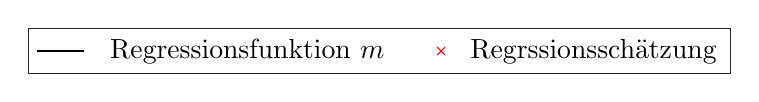
\begin{tikzpicture} 
    \begin{axis}[%
    legend columns=2,
    hide axis,
    xmin=10,
    xmax=50,
    ymin=0,
    ymax=0.4,
    legend style={draw=white!15!black,legend cell align=left,column sep=0.25cm}
    ]
    \addlegendimage{no markers,black}
    \addlegendentry{Regressionsfunktion $m \quad$};
     \addlegendimage{only marks,red,mark=x}
    \addlegendentry{Regrssionsschätzung};
    \end{axis}
\end{tikzpicture}}
    \end{subfigure}
    \caption{Approximation der Regressionsfunktion $m(x) = \sin\big(\frac{\pi}{2} \cdot x^2\big)$ durch unseren Neuronale-Netze-Regressionsschätzer mit Parametern $d = 1$, $q = 2$, $R = 10^6$, $a = 3$, $M = 2$ und $N \in \{2,4,8,16\}$.}
    \label{fig:subfig.a.1}
\end{figure}

\begin{figure}
    \begin{subfigure}[b]{0.5\textwidth}
    \centering
    \scalebox{0.9}{
	\input{Plots_Simulation/mytikz_N2_M2.tex}}
        \label{fig:subfig2n2m2}
    \end{subfigure}
    \begin{subfigure}[b]{0.5\textwidth}
    \centering
     \scalebox{0.9}{
           \input{Plots_Simulation/mytikz_N2_M4.tex}}  
        \label{fig:subfig2n2m4}
    \end{subfigure}
    \hspace{0.1cm}
    \begin{subfigure}[b]{0.5\textwidth}
    \centering
    \scalebox{0.9}{
	% This file was created by tikzplotlib v0.9.0.
\begin{tikzpicture}

\begin{axis}[
tick align=outside,
tick pos=left,
title={$N = 2$, $M = 8$},
x grid style={white!69.0196078431373!black},
xmin=-3.34207441715318, xmax=3.35388433148518,
xtick style={color=black},
y grid style={white!69.0196078431373!black},
ymin=\ymin, ymax=\ymax,
ytick style={color=black}
]
\addplot [only marks, mark=x, draw=red, fill=red, colormap/viridis]
table{%
x                      y
2.76238288932011 -0.260774352562263
-2.97867143721344 1.15689380636718
1.34016626636584 0.335858889485344
-2.34602979642214 0.492956365678858
0.262724949982951 0.103958622208028
0.761496100082008 0.724226013607884
-1.54231724537519 -0.769824363844907
2.48306325147965 -0.0760164784042068
0.733875172149707 0.600400546997855
-1.60983185163084 -0.883066801300895
1.62079312559885 -0.834302049599596
-2.36695752001599 0.359769605701572
0.331351911188067 0.214769014993744
-2.43026358118505 0.00352729073987814
0.485904436050117 0.404465500942523
-1.48211932367887 -0.494609863057067
0.896800847728478 0.885784677105308
1.29496171714908 0.535762802502725
0.145113687411967 0.0418511860536157
0.945128446218661 1.02481717783123
1.87976307195033 -0.796807297666625
1.84507362985819 -0.624253446769536
0.718091952323177 0.718545304431815
-0.293385227275351 0.188586465396323
-0.552300065715795 0.426921917153589
2.24848571942618 1.34311583619364
1.21759039268623 0.675959747027524
-1.89038986575959 -0.495148735176456
0.39439287977558 0.238581965388113
2.45284819380034 0.0137910187765892
-2.09586004651037 0.389185056865272
2.07310605318424 0.305003061257402
1.9212147978921 -0.421955603060901
-0.00395339221299285 -0.0620412061007523
-2.77449689108578 -0.391371316462529
-2.11498496761839 0.465222204835514
2.53583216813203 -0.357839966830502
-2.73507122380883 -0.500719447150897
-0.765007401567843 0.776070098168048
0.714237808352825 0.696920163041861
-1.8183117665159 -0.685607676446936
2.88647854344178 0.291217173595041
-2.06414860173947 0.232740737761275
0.238075170967647 0.0358945664115341
0.708067946079868 0.632760558463181
-1.61406030798178 -0.859056835635599
-0.202146064743951 0.141434703993607
-0.0539488252024247 0.0151761549659135
1.60117425795925 -0.8097990525069
0.80568451664324 0.697822698642747
-0.194699681607962 0.107582779771067
1.00165525916385 0.922331417388326
-0.27973544086681 0.180855035562909
0.154269548048458 -0.0276420048851145
0.951408249350171 0.950991726932469
-1.91282770827683 -0.393115519975016
1.72829730703384 -1.0099085652311
0.617192025230384 0.582515503198186
2.88199731082397 0.376269187788341
-1.66570083881295 -0.858079298485065
-0.202401155000559 0.153856692742747
2.37385081559668 0.372053874302325
0.608600458192729 0.568492855075378
1.35575307509289 0.259174789044995
-0.517979014791838 0.365352075395022
1.10585773098792 1.05856665761879
2.67633017908538 -0.604269353019333
-1.79888360556407 -0.698298983612214
1.84419158326392 -0.662952110115582
2.81722807259938 -0.0946348760886822
-2.91258760942001 0.48042566984495
-1.70874248043343 -0.858196806864326
-2.29573847812122 0.840044118215822
1.60454110644872 -0.934672983213413
-2.5127004843436 -0.354212171204713
2.99048135154545 1.45294729457943
-0.662327904724169 0.577119111344625
2.43121659559824 -0.0681493572289528
-1.86853437900319 -0.541475718025601
-0.354766801066255 0.229609537311848
2.06887091403722 0.288907332758733
0.571618684039537 0.485877520831265
-0.227051419851858 0.171805457057884
0.0758984805427056 -0.111758137591589
0.443313161354085 0.292754933197126
-0.358084754486441 0.223738234552026
-1.83864625365714 -0.622303961827702
-2.31620543124488 0.693804103039226
-2.09263243577911 0.341641523059668
-2.6850542168812 -0.59096088038053
0.352058466381789 0.208152896813525
2.08632608421606 0.389921578988937
-0.845283966455336 0.86249637842132
-2.54813476418509 -0.466901357278878
-0.445653528089303 0.288022047013151
0.612047030832008 0.609078463973348
-0.447579206546175 0.303685518367195
1.86432740164422 -0.749747406491157
2.65131747712023 -0.880356615436864
2.21946463961013 1.12408800099795
1.22399698967933 0.689427711125742
-0.178206451306949 0.103658633355173
1.09618825741951 0.954603753713781
-2.91949013666082 0.537836670833914
2.89486871101226 0.299309291137268
-1.96753600902662 -0.205598887996032
2.43756237577009 -0.158878301786823
1.84265940999664 -0.849286033203679
1.80083810632193 -0.921180704027317
-1.38638365328961 0.137018548535602
-1.68507716545645 -0.86704141832411
-0.427195842515467 0.290443930261047
2.09622660438393 0.354947063153141
-0.297722145169678 0.161894354683285
2.61252068404237 -0.726691112271444
-0.883924036489572 0.908357220950865
0.716352994180558 0.663364018137835
2.88419421813468 0.251096754271755
0.86077513344483 0.899168598149389
-2.72701070375638 -0.525444059870752
-0.218657454289729 0.135885986762933
-0.991491937718017 1.02352011335633
0.193089291130048 -0.00493977140383477
-1.29152274832121 0.566320411508967
-2.26643261861998 1.03964275036918
1.00973393250481 1.01943410903696
1.08815852934784 0.961039557161564
2.20283579999453 1.06103396106744
-2.20571103862358 0.936333570694152
1.79172184966819 -1.01826550898899
1.96061243043077 -0.270747551512453
0.879299614506912 0.867032624282787
-1.7704671253162 -0.766310565438159
-1.43147571356497 -0.145663224773309
-0.489019094764946 0.358225754772378
0.250794436696388 0.134977875397721
-0.135372266446698 0.0574351753628316
-0.195240647727783 0.143741731250259
2.039044261186 0.10422226386461
2.22061419184541 1.19237820185408
1.9005237862606 -0.510568644643307
2.2668085118082 1.28212825244984
0.426052571622439 0.346251187176824
2.78421680003449 -0.358632977776056
0.639266089502806 0.615490424823834
0.623686446478088 0.522089578488886
-1.08421357755229 0.983640219590892
1.08722510470211 0.935937705513695
-2.68820586896783 -0.583233227267607
-2.19272147392835 0.866536735040135
-2.21854699456341 1.02249108241525
0.931207723348414 1.02089024970572
-1.94800444937197 -0.267482534491084
-0.953119060490716 0.969685890399585
-2.73413006500137 -0.513302244237271
-1.59759383930094 -0.845104418743034
2.78534594909577 -0.567344471167497
0.0548364150982064 -0.0961197730034842
-2.09355288917141 0.354015864433495
0.138051190406785 -0.0382552656090519
2.66105630346648 -0.773470115830907
2.194116084038 1.06404499680557
-0.647604786417679 0.511651085249143
-1.29679490415958 0.556418007868288
1.57037917615645 -0.720584526303209
-1.55709405118147 -0.80353863124546
-1.47460587205589 -0.448849223175975
-2.49548187492042 -0.295266793564403
2.18486456858416 1.19556646003826
-0.312606506278321 0.215541446380677
0.370717563659841 0.204600265943954
1.42026574616112 0.015239517981798
1.77893320278717 -0.823221150416053
-0.314951166058117 0.223157426685126
-1.89523466294521 -0.465493735068443
1.97239710916981 -0.108171405797183
-2.81401224103046 -0.214163371491842
2.68036961764771 -1.09475172987415
0.461867078865009 0.404470599533256
2.25233243070412 1.53226046301175
0.651392621841352 0.528914099713153
-1.49004249508606 -0.590304890883481
-1.22322045902457 0.781707426702724
0.197535354189919 0.0209002191346228
2.77246927708256 -0.450280520095304
-1.89302637305893 -0.462312908322321
0.0593902688586541 -0.0791657808010209
-0.937271379378934 0.970892336268786
1.61835206974311 -1.07001001002177
1.81719891859454 -0.818805173539537
-0.4526405381867 0.34026460352423
-1.77526500003398 -0.759001415494696
-2.59746323802687 -0.551802167297634
-1.80811041347663 -0.682407215726837
-1.36559489922371 0.265882901052807
0.592733507455263 0.519517337062177
2.23850098364661 1.41160518169405
-2.23061436692708 1.06818410472445
2.74913245028938 -0.610480815867311
1.09902506312488 0.956986802395602
};
\addplot [semithick, black]
table {%
-3 1
-2.99 0.995576734820054
-2.98 0.982404791977482
-2.97 0.960687140310815
-2.96 0.930698746339696
-2.95 0.892782465918225
-2.94 0.847344438774256
-2.93 0.794849046139829
-2.92 0.735813493407208
-2.91 0.670802080787205
-2.9 0.6004202253259
-2.89 0.525308297382294
-2.88 0.446135333817727
-2.87 0.363592688736647
-2.86 0.278387680690676
-2.85 0.191237292858769
-2.84 0.102861979893671
-2.83 0.0139796319282911
-2.82 -0.0747002572851044
-2.81 -0.162482174923344
-2.8 -0.248689887164819
-2.79 -0.332671415810564
-2.78 -0.413803662790115
-2.77 -0.491496656276015
-2.76000000000001 -0.565197396549224
-2.75000000000001 -0.63439328416361
-2.74000000000001 -0.698615117310616
-2.73000000000001 -0.7574396495474
-2.72000000000001 -0.810491703188593
-2.71000000000001 -0.857445837641644
-2.70000000000001 -0.898027575760592
-2.69000000000001 -0.932014194877928
-2.68000000000001 -0.959235092527838
-2.67000000000001 -0.979571739978357
-2.66000000000001 -0.992957239530362
-2.65000000000001 -0.999375504106505
-2.64000000000001 -0.998860079935072
-2.63000000000001 -0.991492635127341
-2.62000000000001 -0.977401138650261
-2.61000000000001 -0.956757755609883
-2.60000000000001 -0.929776485888277
-2.59000000000001 -0.896710574023413
-2.58000000000001 -0.857849718795458
-2.57000000000001 -0.813517111294285
-2.56000000000001 -0.764066330303094
-2.55000000000001 -0.709878123655345
-2.54000000000001 -0.651357103821107
-2.53000000000001 -0.588928385370132
-2.52000000000001 -0.523034191158988
-2.51000000000001 -0.454130453115695
-2.50000000000001 -0.382683432365167
-2.49000000000001 -0.309166382170306
-2.48000000000001 -0.234056275775223
-2.47000000000001 -0.157830619746354
-2.46000000000001 -0.0809643718325892
-2.45000000000001 -0.00392698072389465
-2.44000000000001 0.072820436603254
-2.43000000000001 0.148827765990005
-2.42000000000001 0.223658403427451
-2.41000000000001 0.296891588141009
-2.40000000000001 0.368124552684589
-2.39000000000001 0.43697448301218
-2.38000000000001 0.503080283168017
-2.37000000000001 0.56610414086275
-2.36000000000001 0.625732891772279
-2.35000000000001 0.681679181898872
-2.34000000000001 0.733682428763456
-2.33000000000001 0.781509583546624
-2.32000000000001 0.824955697558263
-2.31000000000001 0.863844297587357
-2.30000000000001 0.898027575760569
-2.29000000000002 0.927386400518292
-2.28000000000002 0.951830156198068
-2.27000000000002 0.971296419496836
-2.26000000000002 0.985750481765479
-2.25000000000002 0.995184726672186
-2.24000000000002 0.999617873256875
-2.23000000000002 0.999094094789406
-2.22000000000002 0.993682024142277
-2.21000000000002 0.983473656597255
-2.20000000000002 0.96858316112866
-2.19000000000002 0.949145611247931
-2.18000000000002 0.925315646459183
-2.17000000000002 0.897266075268519
-2.16000000000002 0.865186430515806
-2.15000000000002 0.829281487561826
-2.14000000000002 0.789769755571343
-2.13000000000002 0.746881951789148
-2.12000000000002 0.700859468316991
-2.11000000000002 0.651952840469899
-2.10000000000002 0.600420225325985
-2.09000000000002 0.546525898589853
-2.08000000000002 0.490538777371198
-2.07000000000002 0.432730975942088
-2.06000000000002 0.373376400983612
-2.05000000000002 0.31274939226965
-2.04000000000002 0.251123414166708
-2.03000000000002 0.188769802758421
-2.02000000000002 0.125956572835066
-2.01000000000002 0.062947288426061
-2.00000000000002 1.33870012014889e-13
-1.99000000000002 -0.062633749083271
-1.98000000000002 -0.124709844813965
-1.97000000000002 -0.185992451913749
-1.96000000000002 -0.246254789302508
-1.95000000000002 -0.305279831055913
-1.94000000000002 -0.3628609327075
-1.93000000000002 -0.418802383167873
-1.92000000000002 -0.472919882928091
-1.91000000000002 -0.525040949582032
-1.90000000000002 -0.575005252043164
-1.89000000000002 -0.622664875144035
-1.88000000000002 -0.667884516592001
-1.87000000000002 -0.710541618511978
-1.86000000000002 -0.750526436036607
-1.85000000000002 -0.787742045606543
-1.84000000000002 -0.822104295818981
-1.83000000000002 -0.85354170381174
-1.82000000000003 -0.881995300293982
-1.81000000000003 -0.907418426433774
-1.80000000000003 -0.929776485888198
-1.79000000000003 -0.949046655314642
-1.78000000000003 -0.965217556733346
-1.77000000000003 -0.978288895122437
-1.76000000000003 -0.988271064618766
-1.75000000000003 -0.995184726672183
-1.74000000000003 -0.99906036345861
-1.73000000000003 -0.999937809799883
-1.72000000000003 -0.997865766766904
-1.71000000000003 -0.992901300058717
-1.70000000000003 -0.985109326154799
-1.69000000000003 -0.974562089132473
-1.68000000000003 -0.961338630927184
-1.67000000000003 -0.945524257691589
-1.66000000000003 -0.92721000478115
-1.65000000000003 -0.906492102760418
-1.64000000000003 -0.883471446686396
-1.63000000000003 -0.858253070784441
-1.62000000000003 -0.830945630488965
-1.61000000000003 -0.801660893676759
-1.60000000000003 -0.770513242775885
-1.59000000000003 -0.737619189288572
-1.58000000000003 -0.703096902123257
-1.57000000000003 -0.667065750989361
-1.56000000000003 -0.629645865969377
-1.55000000000003 -0.590957714246878
-1.54000000000003 -0.5511216948366
-1.53000000000003 -0.510257752034371
-1.52000000000003 -0.468485008180726
-1.51000000000003 -0.425921416212823
-1.50000000000003 -0.382683432365229
-1.49000000000003 -0.338885709271396
-1.48000000000003 -0.29464080961443
-1.47000000000003 -0.250058940378286
-1.46000000000003 -0.205247707658841
-1.45000000000003 -0.16031189190854
-1.44000000000003 -0.115353243408457
-1.43000000000003 -0.0704702976877775
-1.42000000000003 -0.0257582105426693
-1.41000000000003 0.018691387755514
-1.40000000000003 0.0627905195291638
-1.39000000000003 0.106454968557562
-1.38000000000003 0.149604371296494
-1.37000000000003 0.192162291056312
-1.36000000000003 0.234056275774993
-1.35000000000004 0.275217900052248
-1.34000000000004 0.315582792135412
-1.33000000000004 0.355090646567928
-1.32000000000004 0.393685223226887
-1.31000000000004 0.431314333487567
-1.30000000000004 0.467929814260443
-1.29000000000004 0.503487490649953
-1.28000000000004 0.537947127984647
-1.27000000000004 0.571272373965398
-1.26000000000004 0.603430691672474
-1.25000000000004 0.634393284163532
-1.24000000000004 0.664135011383361
-1.23000000000004 0.692634300092632
-1.22000000000004 0.719873047507249
-1.21000000000004 0.745836519322339
-1.20000000000004 0.770513242775697
-1.19000000000004 0.79389489538482
-1.18000000000004 0.815976189969678
-1.17000000000004 0.836754756550324
-1.16000000000004 0.856231021684473
-1.15000000000004 0.87440808578545
-1.14000000000004 0.891291598935659
-1.13000000000004 0.906889635684947
-1.12000000000004 0.921212569297285
-1.11000000000004 0.93427294588298
-1.10000000000004 0.9460853588275
-1.09000000000004 0.956666323901834
-1.08000000000004 0.966034155413461
-1.07000000000004 0.974208843731348
-1.06000000000004 0.981211934493193
-1.05000000000004 0.987066409778344
-1.04000000000004 0.991796571505593
-1.03000000000004 0.995427927291427
-1.02000000000004 0.997987078981312
-1.01000000000004 0.999501614044331
-1.00000000000004 1
-0.990000000000043 0.999511482025296
-0.980000000000043 0.998065983870084
-0.970000000000043 0.995694012190007
-0.960000000000043 0.992426564387702
-0.950000000000044 0.988295040035889
-0.940000000000044 0.983331155939389
-0.930000000000044 0.977566864877576
-0.920000000000044 0.971034278054095
-0.910000000000045 0.963765591266851
-0.900000000000045 0.955793014798367
-0.890000000000045 0.94714870701456
-0.880000000000045 0.937864711648732
-0.870000000000045 0.927972898737259
-0.860000000000046 0.917504909163832
-0.850000000000046 0.906492102760406
-0.840000000000046 0.894965509904969
-0.830000000000046 0.882955786549018
-0.820000000000046 0.870493172601118
-0.810000000000047 0.857607453587072
-0.800000000000047 0.844327925502078
-0.790000000000047 0.830683362765738
-0.780000000000047 0.816701989186866
-0.770000000000048 0.802411451841723
-0.760000000000048 0.787838797766522
-0.750000000000048 0.773010453362809
-0.740000000000048 0.757952206412552
-0.730000000000048 0.742689190598499
-0.720000000000049 0.727245872424471
-0.710000000000049 0.711646040429847
-0.700000000000049 0.695912796592392
-0.690000000000049 0.68006854981388
-0.680000000000049 0.664135011383549
-0.67000000000005 0.648133192315342
-0.66000000000005 0.632083402456062
-0.65000000000005 0.61600525126299
-0.64000000000005 0.599917650151169
-0.630000000000051 0.583838816312412
-0.620000000000051 0.567786277910133
-0.610000000000051 0.551776880556293
-0.600000000000051 0.535826794979078
-0.590000000000051 0.519951525792427
-0.580000000000052 0.504165921281037
-0.570000000000052 0.488484184117171
-0.560000000000052 0.472919882928293
-0.550000000000052 0.457485964637341
-0.540000000000052 0.442194767500267
-0.530000000000053 0.427058034768333
-0.520000000000053 0.4120869289055
-0.510000000000053 0.397292046294142
-0.500000000000053 0.382683432365167
-0.490000000000054 0.368270597091477
-0.480000000000054 0.354062530786545
-0.470000000000054 0.340067720152659
-0.460000000000054 0.326294164526146
-0.450000000000054 0.312749392269599
-0.440000000000055 0.299440477263786
-0.430000000000055 0.286374055454505
-0.420000000000055 0.273556341412193
-0.410000000000055 0.260993144864562
-0.400000000000055 0.248689887164922
-0.390000000000056 0.23665161766118
-0.380000000000056 0.22488302993274
-0.370000000000056 0.213388477864702
-0.360000000000056 0.202171991530836
-0.350000000000056 0.191237292858801
-0.340000000000057 0.180587811053027
-0.330000000000057 0.170226697752469
-0.320000000000057 0.160156841902239
-0.310000000000057 0.150380884319751
-0.300000000000058 0.140901231937636
-0.290000000000058 0.131720071707145
-0.280000000000058 0.122839384147215
-0.270000000000058 0.114260956525697
-0.260000000000058 0.105986395660502
-0.250000000000059 0.0980171403296064
-0.240000000000059 0.0903544732799798
-0.230000000000059 0.0829995328265039
-0.220000000000059 0.0759533240329385
-0.210000000000059 0.0692167294678623
-0.20000000000006 0.0627905195293508
-0.19000000000006 0.0566753623329036
-0.18000000000006 0.0508718331578319
-0.17000000000006 0.0453804234479493
-0.160000000000061 0.0402015493629836
-0.150000000000061 0.0353355598776498
-0.140000000000061 0.0307827444257893
-0.130000000000061 0.0265433400874004
-0.120000000000061 0.0226175383167529
-0.110000000000062 0.019005491210107
-0.100000000000062 0.0157073173118401
-0.090000000000062 0.012723106958029
-0.0800000000000622 0.0100529271567463
-0.0700000000000625 0.00769682600450373
-0.0600000000000627 0.00565483663842069
-0.0500000000000629 0.00392698072381588
-0.0400000000000631 0.00251327147701166
-0.0300000000000633 0.00141371622321359
-0.0200000000000635 0.000628318489380248
-0.0100000000000637 0.000157079632035528
-6.3948846218409e-14 6.42370078682459e-27
0.00999999999993584 0.00015707963203151
0.0199999999999356 0.000628318489372212
0.0299999999999354 0.00141371622320154
0.0399999999999352 0.00251327147699558
0.049999999999935 0.00392698072379579
0.0599999999999348 0.00565483663839659
0.0699999999999346 0.00769682600447561
0.0799999999999343 0.0100529271567142
0.0899999999999341 0.0127231069579928
0.0999999999999339 0.0157073173117999
0.109999999999934 0.0190054912100628
0.119999999999933 0.0226175383167047
0.129999999999933 0.0265433400873482
0.139999999999933 0.0307827444257331
0.149999999999933 0.0353355598775896
0.159999999999933 0.0402015493629194
0.169999999999932 0.045380423447881
0.179999999999932 0.0508718331577597
0.189999999999932 0.0566753623328273
0.199999999999932 0.0627905195292706
0.209999999999932 0.0692167294677781
0.219999999999931 0.0759533240328503
0.229999999999931 0.0829995328264118
0.239999999999931 0.0903544732798837
0.249999999999931 0.0980171403295065
0.259999999999931 0.105986395660398
0.26999999999993 0.114260956525589
0.27999999999993 0.122839384147103
0.28999999999993 0.131720071707029
0.29999999999993 0.140901231937517
0.309999999999929 0.150380884319628
0.319999999999929 0.160156841902112
0.329999999999929 0.170226697752338
0.339999999999929 0.180587811052893
0.349999999999929 0.191237292858663
0.359999999999928 0.202171991530694
0.369999999999928 0.213388477864557
0.379999999999928 0.224883029932591
0.389999999999928 0.236651617661028
0.399999999999928 0.248689887164767
0.409999999999927 0.260993144864403
0.419999999999927 0.273556341412031
0.429999999999927 0.28637405545434
0.439999999999927 0.299440477263618
0.449999999999926 0.312749392269427
0.459999999999926 0.326294164525971
0.469999999999926 0.340067720152481
0.479999999999926 0.354062530786364
0.489999999999926 0.368270597091294
0.499999999999925 0.382683432364981
0.509999999999925 0.397292046293954
0.519999999999925 0.412086928905309
0.529999999999925 0.42705803476814
0.539999999999925 0.442194767500072
0.549999999999924 0.457485964637144
0.559999999999924 0.472919882928095
0.569999999999924 0.488484184116971
0.579999999999924 0.504165921280836
0.589999999999923 0.519951525792225
0.599999999999923 0.535826794978874
0.609999999999923 0.551776880556088
0.619999999999923 0.567786277909928
0.629999999999923 0.583838816312206
0.639999999999922 0.599917650150963
0.649999999999922 0.616005251262785
0.659999999999922 0.632083402455857
0.669999999999922 0.648133192315137
0.679999999999922 0.664135011383345
0.689999999999921 0.680068549813677
0.699999999999921 0.69591279659219
0.709999999999921 0.711646040429646
0.719999999999921 0.727245872424273
0.72999999999992 0.742689190598303
0.73999999999992 0.757952206412358
0.74999999999992 0.773010453362617
0.75999999999992 0.787838797766334
0.76999999999992 0.802411451841539
0.779999999999919 0.816701989186685
0.789999999999919 0.830683362765561
0.799999999999919 0.844327925501906
0.809999999999919 0.857607453586905
0.819999999999919 0.870493172600956
0.829999999999918 0.882955786548861
0.839999999999918 0.894965509904818
0.849999999999918 0.906492102760262
0.859999999999918 0.917504909163694
0.869999999999918 0.927972898737128
0.879999999999917 0.93786471164861
0.889999999999917 0.947148707014445
0.899999999999917 0.955793014798261
0.909999999999917 0.963765591266753
0.919999999999916 0.971034278054007
0.929999999999916 0.977566864877497
0.939999999999916 0.98333115593932
0.949999999999916 0.988295040035831
0.959999999999916 0.992426564387655
0.969999999999915 0.995694012189971
0.979999999999915 0.99806598387006
0.989999999999915 0.999511482025283
0.999999999999915 1
1.00999999999991 0.999501614044344
1.01999999999991 0.997987078981338
1.02999999999991 0.995427927291467
1.03999999999991 0.991796571505646
1.04999999999991 0.987066409778411
1.05999999999991 0.981211934493276
1.06999999999991 0.974208843731445
1.07999999999991 0.966034155413573
1.08999999999991 0.956666323901962
1.09999999999991 0.946085358827643
1.10999999999991 0.934272945883139
1.11999999999991 0.92121256929746
1.12999999999991 0.906889635685138
1.13999999999991 0.891291598935866
1.14999999999991 0.874408085785674
1.15999999999991 0.856231021684713
1.16999999999991 0.836754756550582
1.17999999999991 0.815976189969952
1.18999999999991 0.793894895385111
1.19999999999991 0.770513242776004
1.20999999999991 0.745836519322663
1.21999999999991 0.719873047507589
1.22999999999991 0.692634300092988
1.23999999999991 0.664135011383733
1.24999999999991 0.63439328416392
1.25999999999991 0.603430691672878
1.26999999999991 0.571272373965817
1.27999999999991 0.537947127985081
1.28999999999991 0.503487490650401
1.29999999999991 0.467929814260904
1.30999999999991 0.431314333488042
1.31999999999991 0.393685223227375
1.32999999999991 0.355090646568427
1.33999999999991 0.315582792135923
1.34999999999991 0.27521790005277
1.35999999999991 0.234056275775525
1.36999999999991 0.192162291056853
1.37999999999991 0.149604371297043
1.38999999999991 0.106454968558117
1.39999999999991 0.0627905195297253
1.40999999999991 0.0186913877560805
1.41999999999991 -0.0257582105420993
1.42999999999991 -0.0704702976872039
1.43999999999991 -0.115353243407883
1.44999999999991 -0.160311891907964
1.4599999999999 -0.205247707658268
1.4699999999999 -0.250058940377715
1.4799999999999 -0.294640809613862
1.4899999999999 -0.338885709270833
1.4999999999999 -0.382683432364672
1.5099999999999 -0.425921416212274
1.5199999999999 -0.468485008180186
1.5299999999999 -0.510257752033843
1.5399999999999 -0.551121694836084
1.5499999999999 -0.590957714246376
1.5599999999999 -0.62964586596889
1.5699999999999 -0.667065750988891
1.5799999999999 -0.703096902122806
1.5899999999999 -0.73761918928814
1.5999999999999 -0.770513242775475
1.6099999999999 -0.801660893676373
1.6199999999999 -0.830945630488602
1.6299999999999 -0.858253070784105
1.6399999999999 -0.883471446686087
1.6499999999999 -0.906492102760138
1.6599999999999 -0.9272100047809
1.6699999999999 -0.945524257691371
1.6799999999999 -0.961338630926998
1.6899999999999 -0.974562089132321
1.6999999999999 -0.985109326154682
1.7099999999999 -0.992901300058635
1.7199999999999 -0.997865766766859
1.7299999999999 -0.999937809799876
1.7399999999999 -0.99906036345864
1.7499999999999 -0.995184726672251
1.7599999999999 -0.988271064618874
1.7699999999999 -0.978288895122584
1.7799999999999 -0.965217556733533
1.7899999999999 -0.949046655314868
1.7999999999999 -0.929776485888465
1.8099999999999 -0.90741842643408
1.8199999999999 -0.881995300294327
1.8299999999999 -0.853541703812123
1.8399999999999 -0.822104295819402
1.8499999999999 -0.787742045607001
1.8599999999999 -0.750526436037101
1.8699999999999 -0.710541618512508
1.8799999999999 -0.667884516592564
1.8899999999999 -0.622664875144629
1.8999999999999 -0.575005252043788
1.9099999999999 -0.525040949582685
1.9199999999999 -0.47291988292877
1.92999999999989 -0.418802383168577
1.93999999999989 -0.362860932708227
1.94999999999989 -0.305279831056659
1.95999999999989 -0.246254789303272
1.96999999999989 -0.185992451914526
1.97999999999989 -0.124709844814754
1.98999999999989 -0.0626337490840697
1.99999999999989 -6.69931457813724e-13
2.00999999999989 0.0629472884252544
2.01999999999989 0.12595657283426
2.02999999999989 0.18876980275762
2.03999999999989 0.251123414165916
2.04999999999989 0.312749392268867
2.05999999999989 0.373376400982844
2.06999999999989 0.432730975941339
2.07999999999989 0.490538777370471
2.08999999999989 0.54652589858915
2.09999999999989 0.600420225325311
2.10999999999989 0.651952840469257
2.11999999999989 0.700859468316383
2.12999999999989 0.746881951788579
2.13999999999989 0.789769755570817
2.14999999999989 0.829281487561343
2.15999999999989 0.865186430515371
2.16999999999989 0.897266075268134
2.17999999999989 0.925315646458851
2.18999999999989 0.949145611247653
2.19999999999989 0.968583161128441
2.20999999999989 0.983473656597094
2.21999999999989 0.993682024142177
2.22999999999989 0.999094094789368
2.23999999999989 0.9996178732569
2.24999999999989 0.995184726672274
2.25999999999989 0.985750481765632
2.26999999999989 0.971296419497053
2.27999999999989 0.951830156198348
2.28999999999989 0.927386400518636
2.29999999999989 0.898027575760974
2.30999999999989 0.863844297587825
2.31999999999989 0.82495569755879
2.32999999999989 0.781509583547208
2.33999999999989 0.733682428764095
2.34999999999989 0.681679181899562
2.35999999999989 0.625732891773019
2.36999999999989 0.566104140863535
2.37999999999989 0.503080283168843
2.38999999999989 0.436974483013044
2.39999999999988 0.368124552685486
2.40999999999988 0.296891588141934
2.41999999999988 0.2236584034284
2.42999999999988 0.148827765990971
2.43999999999988 0.072820436604232
2.44999999999988 -0.00392698072291233
2.45999999999988 -0.0809643718316048
2.46999999999988 -0.157830619745374
2.47999999999988 -0.234056275774253
2.48999999999988 -0.309166382169355
2.49999999999988 -0.382683432364238
2.50999999999988 -0.454130453114798
2.51999999999988 -0.523034191158123
2.52999999999988 -0.58892838536931
2.53999999999988 -0.651357103820333
2.54999999999988 -0.709878123654623
2.55999999999988 -0.764066330302429
2.56999999999988 -0.813517111293685
2.57999999999988 -0.857849718794925
2.58999999999988 -0.896710574022952
2.59999999999988 -0.929776485887892
2.60999999999988 -0.956757755609577
2.61999999999988 -0.977401138650039
2.62999999999988 -0.991492635127203
2.63999999999988 -0.998860079935021
2.64999999999988 -0.999375504106543
2.65999999999988 -0.992957239530489
2.66999999999988 -0.979571739978573
2.67999999999988 -0.959235092528142
2.68999999999988 -0.93201419487832
2.69999999999988 -0.898027575761069
2.70999999999988 -0.857445837642205
2.71999999999988 -0.810491703189233
2.72999999999988 -0.757439649548115
2.73999999999988 -0.698615117311402
2.74999999999988 -0.634393284164464
2.75999999999988 -0.565197396550139
2.76999999999988 -0.491496656276984
2.77999999999988 -0.413803662791132
2.78999999999988 -0.332671415811622
2.79999999999988 -0.248689887165909
2.80999999999988 -0.162482174924459
2.81999999999988 -0.0747002572862345
2.82999999999988 0.0139796319271562
2.83999999999988 0.102861979892536
2.84999999999988 0.191237292857646
2.85999999999988 0.278387680689572
2.86999999999987 0.36359268873557
2.87999999999987 0.44613533381669
2.88999999999987 0.525308297381304
2.89999999999987 0.600420225324967
2.90999999999987 0.670802080786339
2.91999999999987 0.735813493406414
2.92999999999987 0.794849046139114
2.93999999999987 0.847344438773628
2.94999999999987 0.892782465917691
2.95999999999987 0.930698746339261
2.96999999999987 0.960687140310484
2.97999999999987 0.982404791977258
2.98999999999987 0.995576734819941
};
\end{axis}

\end{tikzpicture}
}
        \label{fig:subfig2n2m8}
    \end{subfigure}
    \begin{subfigure}[b]{0.5\textwidth}
    \centering
     \scalebox{0.9}{
           \input{Plots_Simulation/mytikz_N2_M16.tex}}
        \label{fig:subfig2n2m16}
    \end{subfigure}
    \begin{subfigure}[b]{1\textwidth}
        \centering
        \scalebox{0.9}{
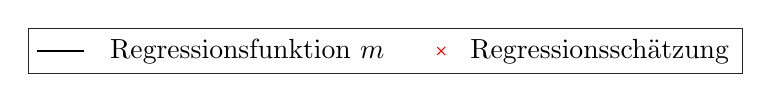
\begin{tikzpicture} 
    \begin{axis}[%
    legend columns=2,
    hide axis,
    xmin=10,
    xmax=50,
    ymin=0,
    ymax=0.4,
    legend style={draw=white!15!black,legend cell align=left,column sep=0.25cm}
    ]
    \addlegendimage{no markers,black}
    \addlegendentry{Regressionsfunktion $m \quad$};
     \addlegendimage{only marks,red,mark=x}
    \addlegendentry{Regressionsschätzung};
    \end{axis}
\end{tikzpicture}}
    \end{subfigure}
     \caption{Approximation der Regressionsfunktion $m(x) = \sin\big(\frac{\pi}{2} \cdot x^2\big)$ durch unseren Neuronale-Netze-Regressionsschätzer mit Parametern $d = 1$, $q = 2$, $R = 10^6$, $a = 3$, $N = 2$ und $M \in \{2,4,8,16\}$.}
\label{fig:subfig.a.2}
\end{figure}
\begin{figure}
    \begin{subfigure}[b]{0.5\textwidth}
    \centering
    \scalebox{0.9}{
	% This file was created by tikzplotlib v0.9.0.
\begin{tikzpicture}

\begin{axis}[
tick align=outside,
tick pos=left,
title={$N = 16$, $M = 2$},
x grid style={white!69.0196078431373!black},
xmin=-3.34207441715318, xmax=3.35388433148518,
xtick style={color=black},
y grid style={white!69.0196078431373!black},
ymin=\ymin, ymax=\ymax,
ytick style={color=black}
]
\addplot [only marks, mark=x, draw=red, fill=red, colormap/viridis]
table{%
x                      y
2.76238288932011 -0.766325584595689
-2.97867143721344 0.945972626392604
1.34016626636584 0.359459037342129
-2.34602979642214 0.796439864331818
0.262724949982951 0.11697884998794
0.761496100082008 0.826019898546403
-1.54231724537519 -0.50444448564422
2.48306325147965 -0.163379516037402
0.733875172149707 0.763973351678569
-1.60983185163084 -0.737120008728139
1.62079312559885 -0.827829522688127
-2.36695752001599 0.674869910004027
0.331351911188067 0.151868986403466
-2.43026358118505 0.239623424197933
0.485904436050117 0.341925938426166
-1.48211932367887 -0.237314469473873
0.896800847728478 0.966034627540416
1.29496171714908 0.480147772472872
0.145113687411967 0.0270108476204783
0.945128446218661 1.01035019990797
1.87976307195033 -0.611683546975155
1.84507362985819 -0.795076304770272
0.718091952323177 0.733965401288443
-0.293385227275351 0.132727176527533
-0.552300065715795 0.45208402171629
2.24848571942618 0.92528092780685
1.21759039268623 0.738609518565516
-1.89038986575959 -0.580111925801957
0.39439287977558 0.258794449086443
2.45284819380034 0.0631130541912442
-2.09586004651037 0.581982610555187
2.07310605318424 0.42472702133845
1.9212147978921 -0.423936952914823
-0.00395339221299285 0.0478843203817596
-2.77449689108578 -0.532245446691913
-2.11498496761839 0.622216094808593
2.53583216813203 -0.45431837588596
-2.73507122380883 -0.955116815815519
-0.765007401567843 0.792719597554144
0.714237808352825 0.710169847835892
-1.8183117665159 -0.873344605318397
2.88647854344178 0.598550513662334
-2.06414860173947 0.448605924099559
0.238075170967647 0.0967925788905418
0.708067946079868 0.729469699813195
-1.61406030798178 -0.823280177876845
-0.202146064743951 0.0295503219242715
-0.0539488252024247 0.0189879243978371
1.60117425795925 -0.774601047946271
0.80568451664324 0.878444379972392
-0.194699681607962 0.036321273210657
1.00165525916385 0.996116103793614
-0.27973544086681 0.114304892851678
0.154269548048458 0.029967596543592
0.951408249350171 0.989994728795778
-1.91282770827683 -0.454529854224978
1.72829730703384 -0.956682599580512
0.617192025230384 0.528943821689262
2.88199731082397 0.489716678801003
-1.66570083881295 -0.988235964670645
-0.202401155000559 0.0378205866162211
2.37385081559668 0.545429174087794
0.608600458192729 0.4976616948579
1.35575307509289 0.268707456301176
-0.517979014791838 0.418078423471025
1.10585773098792 0.923634013933351
2.67633017908538 -0.992814762837324
-1.79888360556407 -0.975392358992915
1.84419158326392 -0.779129508561444
2.81722807259938 -0.247308687468421
-2.91258760942001 0.638235599256928
-1.70874248043343 -1.01675515448634
-2.29573847812122 0.89295432601305
1.60454110644872 -0.767058329116834
-2.5127004843436 -0.364617406018911
2.99048135154545 0.509285880171684
-0.662327904724169 0.603709522380593
2.43121659559824 0.164999565026513
-1.86853437900319 -0.670944349254661
-0.354766801066255 0.21183332735161
2.06887091403722 0.393618615043543
0.571618684039537 0.444241160687973
-0.227051419851858 0.0548993056320555
0.0758984805427056 0.0217118512581678
0.443313161354085 0.338236590005564
-0.358084754486441 0.215830235438439
-1.83864625365714 -0.789129066937444
-2.31620543124488 0.825704007328304
-2.09263243577911 0.577315406796979
-2.6850542168812 -1.10356452806455
0.352058466381789 0.184846101105912
2.08632608421606 0.515960535033473
-0.845283966455336 0.922164978821915
-2.54813476418509 -0.588155479779903
-0.445653528089303 0.34512363386809
0.612047030832008 0.498187881396715
-0.447579206546175 0.352681919329291
1.86432740164422 -0.71777144900056
2.65131747712023 -0.997908502794843
2.21946463961013 0.955484680671926
1.22399698967933 0.72399418807463
-0.178206451306949 0.0214524370649
1.09618825741951 0.952268292280324
-2.91949013666082 0.710074962115307
2.89486871101226 0.650551568902872
-1.96753600902662 -0.133046626465561
2.43756237577009 0.114420336054236
1.84265940999664 -0.803387821191435
1.80083810632193 -0.867443886008529
-1.38638365328961 0.181509613264514
-1.68507716545645 -0.953145642621713
-0.427195842515467 0.318907817229158
2.09622660438393 0.565411542954988
-0.297722145169678 0.136989062006555
2.61252068404237 -0.982579994559999
-0.883924036489572 0.963191537463801
0.716352994180558 0.723410914709831
2.88419421813468 0.550743732995324
0.86077513344483 0.953927730442908
-2.72701070375638 -0.9687746217173
-0.218657454289729 0.0582721735615733
-0.991491937718017 1.00122108227183
0.193089291130048 0.102132836112914
-1.29152274832121 0.493605529607443
-2.26643261861998 0.955343109338322
1.00973393250481 0.992142368266578
1.08815852934784 0.932748403299171
2.20283579999453 0.940178924631622
-2.20571103862358 0.945232995848325
1.79172184966819 -0.94230593934244
1.96061243043077 -0.221001483239006
0.879299614506912 0.956137824195825
-1.7704671253162 -0.9906305765333
-1.43147571356497 -0.0261703171063605
-0.489019094764946 0.394462975611696
0.250794436696388 0.134090872809203
-0.135372266446698 0.00993489840682106
-0.195240647727783 0.0316465469541166
2.039044261186 0.33303048439445
2.22061419184541 0.888731273016752
1.9005237862606 -0.561321326430926
2.2668085118082 0.909945091144731
0.426052571622439 0.298993295373075
2.78421680003449 -0.455526407814202
0.639266089502806 0.569065784128471
0.623686446478088 0.530430122875644
-1.08421357755229 0.925171721659108
1.08722510470211 0.933563939428368
-2.68820586896783 -1.02586908349711
-2.19272147392835 0.890667476085183
-2.21854699456341 0.954828276166595
0.931207723348414 0.986465203989037
-1.94800444937197 -0.267086463176899
-0.953119060490716 0.999529336410753
-2.73413006500137 -0.854823962304677
-1.59759383930094 -0.710123122723663
2.78534594909577 -0.532162046993591
0.0548364150982064 0.0107398402794998
-2.09355288917141 0.526712166030853
0.138051190406785 0.026487017375763
2.66105630346648 -1.060421531295
2.194116084038 0.88615414036398
-0.647604786417679 0.563927118496397
-1.29679490415958 0.461138260089159
1.57037917615645 -0.617982010825825
-1.55709405118147 -0.568729721104781
-1.47460587205589 -0.167275764459825
-2.49548187492042 -0.237791144865769
2.18486456858416 0.956928638490545
-0.312606506278321 0.150467999138229
0.370717563659841 0.209753728278046
1.42026574616112 0.0181787242776163
1.77893320278717 -0.961324549535883
-0.314951166058117 0.157958505650292
-1.89523466294521 -0.542853788375741
1.97239710916981 -0.175369400893344
-2.81401224103046 -0.134481018740555
2.68036961764771 -0.965480585573514
0.461867078865009 0.325158744858177
2.25233243070412 0.926491076161369
0.651392621841352 0.595360983704299
-1.49004249508606 -0.322174343135326
-1.22322045902457 0.674286427889597
0.197535354189919 0.0819004224918271
2.77246927708256 -0.645517948880053
-1.89302637305893 -0.563944936249319
0.0593902688586541 -0.0377340592096357
-0.937271379378934 1.00491030062006
1.61835206974311 -0.818713736861854
1.81719891859454 -0.827064932302617
-0.4526405381867 0.364059298647535
-1.77526500003398 -0.990119656461944
-2.59746323802687 -0.990358557298789
-1.80811041347663 -0.90811047655358
-1.36559489922371 0.228479295987492
0.592733507455263 0.469988997286455
2.23850098364661 0.901108202213205
-2.23061436692708 0.939618664057149
2.74913245028938 -0.817245874810982
1.09902506312488 0.932252472880929
};
\addplot [semithick, black]
table {%
-3 1
-2.99 0.995576734820054
-2.98 0.982404791977482
-2.97 0.960687140310815
-2.96 0.930698746339696
-2.95 0.892782465918225
-2.94 0.847344438774256
-2.93 0.794849046139829
-2.92 0.735813493407208
-2.91 0.670802080787205
-2.9 0.6004202253259
-2.89 0.525308297382294
-2.88 0.446135333817727
-2.87 0.363592688736647
-2.86 0.278387680690676
-2.85 0.191237292858769
-2.84 0.102861979893671
-2.83 0.0139796319282911
-2.82 -0.0747002572851044
-2.81 -0.162482174923344
-2.8 -0.248689887164819
-2.79 -0.332671415810564
-2.78 -0.413803662790115
-2.77 -0.491496656276015
-2.76000000000001 -0.565197396549224
-2.75000000000001 -0.63439328416361
-2.74000000000001 -0.698615117310616
-2.73000000000001 -0.7574396495474
-2.72000000000001 -0.810491703188593
-2.71000000000001 -0.857445837641644
-2.70000000000001 -0.898027575760592
-2.69000000000001 -0.932014194877928
-2.68000000000001 -0.959235092527838
-2.67000000000001 -0.979571739978357
-2.66000000000001 -0.992957239530362
-2.65000000000001 -0.999375504106505
-2.64000000000001 -0.998860079935072
-2.63000000000001 -0.991492635127341
-2.62000000000001 -0.977401138650261
-2.61000000000001 -0.956757755609883
-2.60000000000001 -0.929776485888277
-2.59000000000001 -0.896710574023413
-2.58000000000001 -0.857849718795458
-2.57000000000001 -0.813517111294285
-2.56000000000001 -0.764066330303094
-2.55000000000001 -0.709878123655345
-2.54000000000001 -0.651357103821107
-2.53000000000001 -0.588928385370132
-2.52000000000001 -0.523034191158988
-2.51000000000001 -0.454130453115695
-2.50000000000001 -0.382683432365167
-2.49000000000001 -0.309166382170306
-2.48000000000001 -0.234056275775223
-2.47000000000001 -0.157830619746354
-2.46000000000001 -0.0809643718325892
-2.45000000000001 -0.00392698072389465
-2.44000000000001 0.072820436603254
-2.43000000000001 0.148827765990005
-2.42000000000001 0.223658403427451
-2.41000000000001 0.296891588141009
-2.40000000000001 0.368124552684589
-2.39000000000001 0.43697448301218
-2.38000000000001 0.503080283168017
-2.37000000000001 0.56610414086275
-2.36000000000001 0.625732891772279
-2.35000000000001 0.681679181898872
-2.34000000000001 0.733682428763456
-2.33000000000001 0.781509583546624
-2.32000000000001 0.824955697558263
-2.31000000000001 0.863844297587357
-2.30000000000001 0.898027575760569
-2.29000000000002 0.927386400518292
-2.28000000000002 0.951830156198068
-2.27000000000002 0.971296419496836
-2.26000000000002 0.985750481765479
-2.25000000000002 0.995184726672186
-2.24000000000002 0.999617873256875
-2.23000000000002 0.999094094789406
-2.22000000000002 0.993682024142277
-2.21000000000002 0.983473656597255
-2.20000000000002 0.96858316112866
-2.19000000000002 0.949145611247931
-2.18000000000002 0.925315646459183
-2.17000000000002 0.897266075268519
-2.16000000000002 0.865186430515806
-2.15000000000002 0.829281487561826
-2.14000000000002 0.789769755571343
-2.13000000000002 0.746881951789148
-2.12000000000002 0.700859468316991
-2.11000000000002 0.651952840469899
-2.10000000000002 0.600420225325985
-2.09000000000002 0.546525898589853
-2.08000000000002 0.490538777371198
-2.07000000000002 0.432730975942088
-2.06000000000002 0.373376400983612
-2.05000000000002 0.31274939226965
-2.04000000000002 0.251123414166708
-2.03000000000002 0.188769802758421
-2.02000000000002 0.125956572835066
-2.01000000000002 0.062947288426061
-2.00000000000002 1.33870012014889e-13
-1.99000000000002 -0.062633749083271
-1.98000000000002 -0.124709844813965
-1.97000000000002 -0.185992451913749
-1.96000000000002 -0.246254789302508
-1.95000000000002 -0.305279831055913
-1.94000000000002 -0.3628609327075
-1.93000000000002 -0.418802383167873
-1.92000000000002 -0.472919882928091
-1.91000000000002 -0.525040949582032
-1.90000000000002 -0.575005252043164
-1.89000000000002 -0.622664875144035
-1.88000000000002 -0.667884516592001
-1.87000000000002 -0.710541618511978
-1.86000000000002 -0.750526436036607
-1.85000000000002 -0.787742045606543
-1.84000000000002 -0.822104295818981
-1.83000000000002 -0.85354170381174
-1.82000000000003 -0.881995300293982
-1.81000000000003 -0.907418426433774
-1.80000000000003 -0.929776485888198
-1.79000000000003 -0.949046655314642
-1.78000000000003 -0.965217556733346
-1.77000000000003 -0.978288895122437
-1.76000000000003 -0.988271064618766
-1.75000000000003 -0.995184726672183
-1.74000000000003 -0.99906036345861
-1.73000000000003 -0.999937809799883
-1.72000000000003 -0.997865766766904
-1.71000000000003 -0.992901300058717
-1.70000000000003 -0.985109326154799
-1.69000000000003 -0.974562089132473
-1.68000000000003 -0.961338630927184
-1.67000000000003 -0.945524257691589
-1.66000000000003 -0.92721000478115
-1.65000000000003 -0.906492102760418
-1.64000000000003 -0.883471446686396
-1.63000000000003 -0.858253070784441
-1.62000000000003 -0.830945630488965
-1.61000000000003 -0.801660893676759
-1.60000000000003 -0.770513242775885
-1.59000000000003 -0.737619189288572
-1.58000000000003 -0.703096902123257
-1.57000000000003 -0.667065750989361
-1.56000000000003 -0.629645865969377
-1.55000000000003 -0.590957714246878
-1.54000000000003 -0.5511216948366
-1.53000000000003 -0.510257752034371
-1.52000000000003 -0.468485008180726
-1.51000000000003 -0.425921416212823
-1.50000000000003 -0.382683432365229
-1.49000000000003 -0.338885709271396
-1.48000000000003 -0.29464080961443
-1.47000000000003 -0.250058940378286
-1.46000000000003 -0.205247707658841
-1.45000000000003 -0.16031189190854
-1.44000000000003 -0.115353243408457
-1.43000000000003 -0.0704702976877775
-1.42000000000003 -0.0257582105426693
-1.41000000000003 0.018691387755514
-1.40000000000003 0.0627905195291638
-1.39000000000003 0.106454968557562
-1.38000000000003 0.149604371296494
-1.37000000000003 0.192162291056312
-1.36000000000003 0.234056275774993
-1.35000000000004 0.275217900052248
-1.34000000000004 0.315582792135412
-1.33000000000004 0.355090646567928
-1.32000000000004 0.393685223226887
-1.31000000000004 0.431314333487567
-1.30000000000004 0.467929814260443
-1.29000000000004 0.503487490649953
-1.28000000000004 0.537947127984647
-1.27000000000004 0.571272373965398
-1.26000000000004 0.603430691672474
-1.25000000000004 0.634393284163532
-1.24000000000004 0.664135011383361
-1.23000000000004 0.692634300092632
-1.22000000000004 0.719873047507249
-1.21000000000004 0.745836519322339
-1.20000000000004 0.770513242775697
-1.19000000000004 0.79389489538482
-1.18000000000004 0.815976189969678
-1.17000000000004 0.836754756550324
-1.16000000000004 0.856231021684473
-1.15000000000004 0.87440808578545
-1.14000000000004 0.891291598935659
-1.13000000000004 0.906889635684947
-1.12000000000004 0.921212569297285
-1.11000000000004 0.93427294588298
-1.10000000000004 0.9460853588275
-1.09000000000004 0.956666323901834
-1.08000000000004 0.966034155413461
-1.07000000000004 0.974208843731348
-1.06000000000004 0.981211934493193
-1.05000000000004 0.987066409778344
-1.04000000000004 0.991796571505593
-1.03000000000004 0.995427927291427
-1.02000000000004 0.997987078981312
-1.01000000000004 0.999501614044331
-1.00000000000004 1
-0.990000000000043 0.999511482025296
-0.980000000000043 0.998065983870084
-0.970000000000043 0.995694012190007
-0.960000000000043 0.992426564387702
-0.950000000000044 0.988295040035889
-0.940000000000044 0.983331155939389
-0.930000000000044 0.977566864877576
-0.920000000000044 0.971034278054095
-0.910000000000045 0.963765591266851
-0.900000000000045 0.955793014798367
-0.890000000000045 0.94714870701456
-0.880000000000045 0.937864711648732
-0.870000000000045 0.927972898737259
-0.860000000000046 0.917504909163832
-0.850000000000046 0.906492102760406
-0.840000000000046 0.894965509904969
-0.830000000000046 0.882955786549018
-0.820000000000046 0.870493172601118
-0.810000000000047 0.857607453587072
-0.800000000000047 0.844327925502078
-0.790000000000047 0.830683362765738
-0.780000000000047 0.816701989186866
-0.770000000000048 0.802411451841723
-0.760000000000048 0.787838797766522
-0.750000000000048 0.773010453362809
-0.740000000000048 0.757952206412552
-0.730000000000048 0.742689190598499
-0.720000000000049 0.727245872424471
-0.710000000000049 0.711646040429847
-0.700000000000049 0.695912796592392
-0.690000000000049 0.68006854981388
-0.680000000000049 0.664135011383549
-0.67000000000005 0.648133192315342
-0.66000000000005 0.632083402456062
-0.65000000000005 0.61600525126299
-0.64000000000005 0.599917650151169
-0.630000000000051 0.583838816312412
-0.620000000000051 0.567786277910133
-0.610000000000051 0.551776880556293
-0.600000000000051 0.535826794979078
-0.590000000000051 0.519951525792427
-0.580000000000052 0.504165921281037
-0.570000000000052 0.488484184117171
-0.560000000000052 0.472919882928293
-0.550000000000052 0.457485964637341
-0.540000000000052 0.442194767500267
-0.530000000000053 0.427058034768333
-0.520000000000053 0.4120869289055
-0.510000000000053 0.397292046294142
-0.500000000000053 0.382683432365167
-0.490000000000054 0.368270597091477
-0.480000000000054 0.354062530786545
-0.470000000000054 0.340067720152659
-0.460000000000054 0.326294164526146
-0.450000000000054 0.312749392269599
-0.440000000000055 0.299440477263786
-0.430000000000055 0.286374055454505
-0.420000000000055 0.273556341412193
-0.410000000000055 0.260993144864562
-0.400000000000055 0.248689887164922
-0.390000000000056 0.23665161766118
-0.380000000000056 0.22488302993274
-0.370000000000056 0.213388477864702
-0.360000000000056 0.202171991530836
-0.350000000000056 0.191237292858801
-0.340000000000057 0.180587811053027
-0.330000000000057 0.170226697752469
-0.320000000000057 0.160156841902239
-0.310000000000057 0.150380884319751
-0.300000000000058 0.140901231937636
-0.290000000000058 0.131720071707145
-0.280000000000058 0.122839384147215
-0.270000000000058 0.114260956525697
-0.260000000000058 0.105986395660502
-0.250000000000059 0.0980171403296064
-0.240000000000059 0.0903544732799798
-0.230000000000059 0.0829995328265039
-0.220000000000059 0.0759533240329385
-0.210000000000059 0.0692167294678623
-0.20000000000006 0.0627905195293508
-0.19000000000006 0.0566753623329036
-0.18000000000006 0.0508718331578319
-0.17000000000006 0.0453804234479493
-0.160000000000061 0.0402015493629836
-0.150000000000061 0.0353355598776498
-0.140000000000061 0.0307827444257893
-0.130000000000061 0.0265433400874004
-0.120000000000061 0.0226175383167529
-0.110000000000062 0.019005491210107
-0.100000000000062 0.0157073173118401
-0.090000000000062 0.012723106958029
-0.0800000000000622 0.0100529271567463
-0.0700000000000625 0.00769682600450373
-0.0600000000000627 0.00565483663842069
-0.0500000000000629 0.00392698072381588
-0.0400000000000631 0.00251327147701166
-0.0300000000000633 0.00141371622321359
-0.0200000000000635 0.000628318489380248
-0.0100000000000637 0.000157079632035528
-6.3948846218409e-14 6.42370078682459e-27
0.00999999999993584 0.00015707963203151
0.0199999999999356 0.000628318489372212
0.0299999999999354 0.00141371622320154
0.0399999999999352 0.00251327147699558
0.049999999999935 0.00392698072379579
0.0599999999999348 0.00565483663839659
0.0699999999999346 0.00769682600447561
0.0799999999999343 0.0100529271567142
0.0899999999999341 0.0127231069579928
0.0999999999999339 0.0157073173117999
0.109999999999934 0.0190054912100628
0.119999999999933 0.0226175383167047
0.129999999999933 0.0265433400873482
0.139999999999933 0.0307827444257331
0.149999999999933 0.0353355598775896
0.159999999999933 0.0402015493629194
0.169999999999932 0.045380423447881
0.179999999999932 0.0508718331577597
0.189999999999932 0.0566753623328273
0.199999999999932 0.0627905195292706
0.209999999999932 0.0692167294677781
0.219999999999931 0.0759533240328503
0.229999999999931 0.0829995328264118
0.239999999999931 0.0903544732798837
0.249999999999931 0.0980171403295065
0.259999999999931 0.105986395660398
0.26999999999993 0.114260956525589
0.27999999999993 0.122839384147103
0.28999999999993 0.131720071707029
0.29999999999993 0.140901231937517
0.309999999999929 0.150380884319628
0.319999999999929 0.160156841902112
0.329999999999929 0.170226697752338
0.339999999999929 0.180587811052893
0.349999999999929 0.191237292858663
0.359999999999928 0.202171991530694
0.369999999999928 0.213388477864557
0.379999999999928 0.224883029932591
0.389999999999928 0.236651617661028
0.399999999999928 0.248689887164767
0.409999999999927 0.260993144864403
0.419999999999927 0.273556341412031
0.429999999999927 0.28637405545434
0.439999999999927 0.299440477263618
0.449999999999926 0.312749392269427
0.459999999999926 0.326294164525971
0.469999999999926 0.340067720152481
0.479999999999926 0.354062530786364
0.489999999999926 0.368270597091294
0.499999999999925 0.382683432364981
0.509999999999925 0.397292046293954
0.519999999999925 0.412086928905309
0.529999999999925 0.42705803476814
0.539999999999925 0.442194767500072
0.549999999999924 0.457485964637144
0.559999999999924 0.472919882928095
0.569999999999924 0.488484184116971
0.579999999999924 0.504165921280836
0.589999999999923 0.519951525792225
0.599999999999923 0.535826794978874
0.609999999999923 0.551776880556088
0.619999999999923 0.567786277909928
0.629999999999923 0.583838816312206
0.639999999999922 0.599917650150963
0.649999999999922 0.616005251262785
0.659999999999922 0.632083402455857
0.669999999999922 0.648133192315137
0.679999999999922 0.664135011383345
0.689999999999921 0.680068549813677
0.699999999999921 0.69591279659219
0.709999999999921 0.711646040429646
0.719999999999921 0.727245872424273
0.72999999999992 0.742689190598303
0.73999999999992 0.757952206412358
0.74999999999992 0.773010453362617
0.75999999999992 0.787838797766334
0.76999999999992 0.802411451841539
0.779999999999919 0.816701989186685
0.789999999999919 0.830683362765561
0.799999999999919 0.844327925501906
0.809999999999919 0.857607453586905
0.819999999999919 0.870493172600956
0.829999999999918 0.882955786548861
0.839999999999918 0.894965509904818
0.849999999999918 0.906492102760262
0.859999999999918 0.917504909163694
0.869999999999918 0.927972898737128
0.879999999999917 0.93786471164861
0.889999999999917 0.947148707014445
0.899999999999917 0.955793014798261
0.909999999999917 0.963765591266753
0.919999999999916 0.971034278054007
0.929999999999916 0.977566864877497
0.939999999999916 0.98333115593932
0.949999999999916 0.988295040035831
0.959999999999916 0.992426564387655
0.969999999999915 0.995694012189971
0.979999999999915 0.99806598387006
0.989999999999915 0.999511482025283
0.999999999999915 1
1.00999999999991 0.999501614044344
1.01999999999991 0.997987078981338
1.02999999999991 0.995427927291467
1.03999999999991 0.991796571505646
1.04999999999991 0.987066409778411
1.05999999999991 0.981211934493276
1.06999999999991 0.974208843731445
1.07999999999991 0.966034155413573
1.08999999999991 0.956666323901962
1.09999999999991 0.946085358827643
1.10999999999991 0.934272945883139
1.11999999999991 0.92121256929746
1.12999999999991 0.906889635685138
1.13999999999991 0.891291598935866
1.14999999999991 0.874408085785674
1.15999999999991 0.856231021684713
1.16999999999991 0.836754756550582
1.17999999999991 0.815976189969952
1.18999999999991 0.793894895385111
1.19999999999991 0.770513242776004
1.20999999999991 0.745836519322663
1.21999999999991 0.719873047507589
1.22999999999991 0.692634300092988
1.23999999999991 0.664135011383733
1.24999999999991 0.63439328416392
1.25999999999991 0.603430691672878
1.26999999999991 0.571272373965817
1.27999999999991 0.537947127985081
1.28999999999991 0.503487490650401
1.29999999999991 0.467929814260904
1.30999999999991 0.431314333488042
1.31999999999991 0.393685223227375
1.32999999999991 0.355090646568427
1.33999999999991 0.315582792135923
1.34999999999991 0.27521790005277
1.35999999999991 0.234056275775525
1.36999999999991 0.192162291056853
1.37999999999991 0.149604371297043
1.38999999999991 0.106454968558117
1.39999999999991 0.0627905195297253
1.40999999999991 0.0186913877560805
1.41999999999991 -0.0257582105420993
1.42999999999991 -0.0704702976872039
1.43999999999991 -0.115353243407883
1.44999999999991 -0.160311891907964
1.4599999999999 -0.205247707658268
1.4699999999999 -0.250058940377715
1.4799999999999 -0.294640809613862
1.4899999999999 -0.338885709270833
1.4999999999999 -0.382683432364672
1.5099999999999 -0.425921416212274
1.5199999999999 -0.468485008180186
1.5299999999999 -0.510257752033843
1.5399999999999 -0.551121694836084
1.5499999999999 -0.590957714246376
1.5599999999999 -0.62964586596889
1.5699999999999 -0.667065750988891
1.5799999999999 -0.703096902122806
1.5899999999999 -0.73761918928814
1.5999999999999 -0.770513242775475
1.6099999999999 -0.801660893676373
1.6199999999999 -0.830945630488602
1.6299999999999 -0.858253070784105
1.6399999999999 -0.883471446686087
1.6499999999999 -0.906492102760138
1.6599999999999 -0.9272100047809
1.6699999999999 -0.945524257691371
1.6799999999999 -0.961338630926998
1.6899999999999 -0.974562089132321
1.6999999999999 -0.985109326154682
1.7099999999999 -0.992901300058635
1.7199999999999 -0.997865766766859
1.7299999999999 -0.999937809799876
1.7399999999999 -0.99906036345864
1.7499999999999 -0.995184726672251
1.7599999999999 -0.988271064618874
1.7699999999999 -0.978288895122584
1.7799999999999 -0.965217556733533
1.7899999999999 -0.949046655314868
1.7999999999999 -0.929776485888465
1.8099999999999 -0.90741842643408
1.8199999999999 -0.881995300294327
1.8299999999999 -0.853541703812123
1.8399999999999 -0.822104295819402
1.8499999999999 -0.787742045607001
1.8599999999999 -0.750526436037101
1.8699999999999 -0.710541618512508
1.8799999999999 -0.667884516592564
1.8899999999999 -0.622664875144629
1.8999999999999 -0.575005252043788
1.9099999999999 -0.525040949582685
1.9199999999999 -0.47291988292877
1.92999999999989 -0.418802383168577
1.93999999999989 -0.362860932708227
1.94999999999989 -0.305279831056659
1.95999999999989 -0.246254789303272
1.96999999999989 -0.185992451914526
1.97999999999989 -0.124709844814754
1.98999999999989 -0.0626337490840697
1.99999999999989 -6.69931457813724e-13
2.00999999999989 0.0629472884252544
2.01999999999989 0.12595657283426
2.02999999999989 0.18876980275762
2.03999999999989 0.251123414165916
2.04999999999989 0.312749392268867
2.05999999999989 0.373376400982844
2.06999999999989 0.432730975941339
2.07999999999989 0.490538777370471
2.08999999999989 0.54652589858915
2.09999999999989 0.600420225325311
2.10999999999989 0.651952840469257
2.11999999999989 0.700859468316383
2.12999999999989 0.746881951788579
2.13999999999989 0.789769755570817
2.14999999999989 0.829281487561343
2.15999999999989 0.865186430515371
2.16999999999989 0.897266075268134
2.17999999999989 0.925315646458851
2.18999999999989 0.949145611247653
2.19999999999989 0.968583161128441
2.20999999999989 0.983473656597094
2.21999999999989 0.993682024142177
2.22999999999989 0.999094094789368
2.23999999999989 0.9996178732569
2.24999999999989 0.995184726672274
2.25999999999989 0.985750481765632
2.26999999999989 0.971296419497053
2.27999999999989 0.951830156198348
2.28999999999989 0.927386400518636
2.29999999999989 0.898027575760974
2.30999999999989 0.863844297587825
2.31999999999989 0.82495569755879
2.32999999999989 0.781509583547208
2.33999999999989 0.733682428764095
2.34999999999989 0.681679181899562
2.35999999999989 0.625732891773019
2.36999999999989 0.566104140863535
2.37999999999989 0.503080283168843
2.38999999999989 0.436974483013044
2.39999999999988 0.368124552685486
2.40999999999988 0.296891588141934
2.41999999999988 0.2236584034284
2.42999999999988 0.148827765990971
2.43999999999988 0.072820436604232
2.44999999999988 -0.00392698072291233
2.45999999999988 -0.0809643718316048
2.46999999999988 -0.157830619745374
2.47999999999988 -0.234056275774253
2.48999999999988 -0.309166382169355
2.49999999999988 -0.382683432364238
2.50999999999988 -0.454130453114798
2.51999999999988 -0.523034191158123
2.52999999999988 -0.58892838536931
2.53999999999988 -0.651357103820333
2.54999999999988 -0.709878123654623
2.55999999999988 -0.764066330302429
2.56999999999988 -0.813517111293685
2.57999999999988 -0.857849718794925
2.58999999999988 -0.896710574022952
2.59999999999988 -0.929776485887892
2.60999999999988 -0.956757755609577
2.61999999999988 -0.977401138650039
2.62999999999988 -0.991492635127203
2.63999999999988 -0.998860079935021
2.64999999999988 -0.999375504106543
2.65999999999988 -0.992957239530489
2.66999999999988 -0.979571739978573
2.67999999999988 -0.959235092528142
2.68999999999988 -0.93201419487832
2.69999999999988 -0.898027575761069
2.70999999999988 -0.857445837642205
2.71999999999988 -0.810491703189233
2.72999999999988 -0.757439649548115
2.73999999999988 -0.698615117311402
2.74999999999988 -0.634393284164464
2.75999999999988 -0.565197396550139
2.76999999999988 -0.491496656276984
2.77999999999988 -0.413803662791132
2.78999999999988 -0.332671415811622
2.79999999999988 -0.248689887165909
2.80999999999988 -0.162482174924459
2.81999999999988 -0.0747002572862345
2.82999999999988 0.0139796319271562
2.83999999999988 0.102861979892536
2.84999999999988 0.191237292857646
2.85999999999988 0.278387680689572
2.86999999999987 0.36359268873557
2.87999999999987 0.44613533381669
2.88999999999987 0.525308297381304
2.89999999999987 0.600420225324967
2.90999999999987 0.670802080786339
2.91999999999987 0.735813493406414
2.92999999999987 0.794849046139114
2.93999999999987 0.847344438773628
2.94999999999987 0.892782465917691
2.95999999999987 0.930698746339261
2.96999999999987 0.960687140310484
2.97999999999987 0.982404791977258
2.98999999999987 0.995576734819941
};
\end{axis}

\end{tikzpicture}
}
        \label{fig:subfig3n16m2}
    \end{subfigure}
    \begin{subfigure}[b]{0.5\textwidth}
    \centering
     \scalebox{0.9}{
           \input{Plots_Simulation/mytikz_N16_M4.tex}}
        \label{fig:subfig3n16m4}
    \end{subfigure}
    \hspace{0.1cm}
    \begin{subfigure}[b]{0.5\textwidth}
    \centering
    \scalebox{0.9}{
	\input{Plots_Simulation/mytikz_N16_M8.tex}}
        \label{fig:subfign3n16m8}
    \end{subfigure}
    \begin{subfigure}[b]{0.5\textwidth}
    \centering
     \scalebox{0.9}{
           \input{Plots_Simulation/mytikz_N16_M16.tex}}
        \label{fig:subfig3n16m16}
    \end{subfigure}
\begin{subfigure}[b]{1\textwidth}
        \centering
        \scalebox{0.9}{
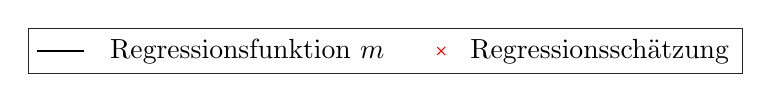
\begin{tikzpicture} 
    \begin{axis}[%
    legend columns=2,
    hide axis,
    xmin=10,
    xmax=50,
    ymin=0,
    ymax=0.4,
    legend style={draw=white!15!black,legend cell align=left,column sep=0.25cm}
    ]
    \addlegendimage{no markers,black}
    \addlegendentry{Regressionsfunktion $m \quad$};
     \addlegendimage{only marks,red,mark=x}
    \addlegendentry{Regressionsschätzung};
    \end{axis}
\end{tikzpicture}}
    \end{subfigure}
 \caption{Approximation der Regressionsfunktion $m(x) = \sin\big(\frac{\pi}{2} \cdot x^2\big)$ durch unseren Neuronale-Netze-Regressionsschätzer mit Parametern $d = 1$, $q = 2$, $R = 10^6$, $a = 3$, $N = 16$ und $M \in \{2,4,8,16\}$.}
 \label{fig:subfig.a.3}
\end{figure}
\begin{figure}
    \begin{subfigure}[b]{0.5\textwidth}
        \centering
        \scalebox{0.9}{
          \input{Plots_Simulation/mytikz_N2_M16.tex}}
        \label{fig:subfig4n2m16}
    \end{subfigure}
    \begin{subfigure}[b]{0.5\textwidth}
    \centering
    \scalebox{0.9}{
           \input{Plots_Simulation/mytikz_N4_M16.tex}}
        \label{fig:subfig4n4m16}
    \end{subfigure}
       \hspace{0.1cm}
    \begin{subfigure}[b]{0.5\textwidth}
    \centering
    \scalebox{0.9}{
	\input{Plots_Simulation/mytikz_N8_M16.tex}}
        \label{fig:subfig4n8m16}
    \end{subfigure}
    \begin{subfigure}[b]{0.5\textwidth}
    \centering
     \scalebox{0.9}{
           \input{Plots_Simulation/mytikz_N16_M16.tex}}
        \label{fig:subfig4n16m16}
    \end{subfigure}
    \begin{subfigure}[b]{1\textwidth}
        \centering
        \scalebox{0.9}{
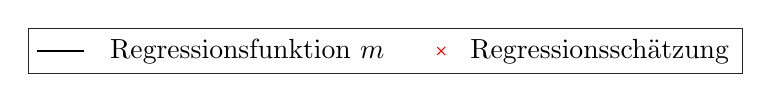
\begin{tikzpicture} 
    \begin{axis}[%
    legend columns=2,
    hide axis,
    xmin=10,
    xmax=50,
    ymin=0,
    ymax=0.4,
    legend style={draw=white!15!black,legend cell align=left,column sep=0.25cm}
    ]
    \addlegendimage{no markers,black}
    \addlegendentry{Regressionsfunktion $m \quad$};
     \addlegendimage{only marks,red,mark=x}
    \addlegendentry{Regressionsschätzung};
    \end{axis}
\end{tikzpicture}}
    \end{subfigure}
     \caption{Approximation der Regressionsfunktion $m(x) = \sin\big(\frac{\pi}{2} \cdot x^2\big)$ durch unseren Neuronale-Netze-Regressionsschätzer mit Parametern $d = 1$, $q = 2$, $R = 10^6$, $a = 3$, $M = 16$ und $N \in \{2,4,8,16\}$.}
    \label{fig:subfig.a.4}
\end{figure}
\begin{figure}
    \begin{subfigure}[b]{0.5\textwidth}
        \centering
        \scalebox{0.9}{
          \input{Plots_Simulation/mytikz_N2_M16.tex}}
          \label{test2}
    \end{subfigure}
    \begin{subfigure}[b]{0.5\textwidth}
    \centering
    \scalebox{0.9}{
           \input{Plots_Simulation/mytikz_N4_M9.tex}}
           \label{fig:test}
    \end{subfigure}
       \hspace{0.1cm}
    \begin{subfigure}[b]{0.5\textwidth}
    \centering
    \scalebox{0.9}{
	\input{Plots_Simulation/mytikz_N9_M4.tex}}
	\label{teat1}
    \end{subfigure}
    \begin{subfigure}[b]{0.5\textwidth}
    \centering
     \scalebox{0.9}{
           % This file was created by tikzplotlib v0.9.0.
\begin{tikzpicture}

\begin{axis}[
tick align=outside,
tick pos=left,
title={$N = 16$, $M = 2$},
x grid style={white!69.0196078431373!black},
xmin=-3.34207441715318, xmax=3.35388433148518,
xtick style={color=black},
y grid style={white!69.0196078431373!black},
ymin=\ymin, ymax=\ymax,
ytick style={color=black}
]
\addplot [only marks, mark=x, draw=red, fill=red, colormap/viridis]
table{%
x                      y
2.76238288932011 -0.766325584595689
-2.97867143721344 0.945972626392604
1.34016626636584 0.359459037342129
-2.34602979642214 0.796439864331818
0.262724949982951 0.11697884998794
0.761496100082008 0.826019898546403
-1.54231724537519 -0.50444448564422
2.48306325147965 -0.163379516037402
0.733875172149707 0.763973351678569
-1.60983185163084 -0.737120008728139
1.62079312559885 -0.827829522688127
-2.36695752001599 0.674869910004027
0.331351911188067 0.151868986403466
-2.43026358118505 0.239623424197933
0.485904436050117 0.341925938426166
-1.48211932367887 -0.237314469473873
0.896800847728478 0.966034627540416
1.29496171714908 0.480147772472872
0.145113687411967 0.0270108476204783
0.945128446218661 1.01035019990797
1.87976307195033 -0.611683546975155
1.84507362985819 -0.795076304770272
0.718091952323177 0.733965401288443
-0.293385227275351 0.132727176527533
-0.552300065715795 0.45208402171629
2.24848571942618 0.92528092780685
1.21759039268623 0.738609518565516
-1.89038986575959 -0.580111925801957
0.39439287977558 0.258794449086443
2.45284819380034 0.0631130541912442
-2.09586004651037 0.581982610555187
2.07310605318424 0.42472702133845
1.9212147978921 -0.423936952914823
-0.00395339221299285 0.0478843203817596
-2.77449689108578 -0.532245446691913
-2.11498496761839 0.622216094808593
2.53583216813203 -0.45431837588596
-2.73507122380883 -0.955116815815519
-0.765007401567843 0.792719597554144
0.714237808352825 0.710169847835892
-1.8183117665159 -0.873344605318397
2.88647854344178 0.598550513662334
-2.06414860173947 0.448605924099559
0.238075170967647 0.0967925788905418
0.708067946079868 0.729469699813195
-1.61406030798178 -0.823280177876845
-0.202146064743951 0.0295503219242715
-0.0539488252024247 0.0189879243978371
1.60117425795925 -0.774601047946271
0.80568451664324 0.878444379972392
-0.194699681607962 0.036321273210657
1.00165525916385 0.996116103793614
-0.27973544086681 0.114304892851678
0.154269548048458 0.029967596543592
0.951408249350171 0.989994728795778
-1.91282770827683 -0.454529854224978
1.72829730703384 -0.956682599580512
0.617192025230384 0.528943821689262
2.88199731082397 0.489716678801003
-1.66570083881295 -0.988235964670645
-0.202401155000559 0.0378205866162211
2.37385081559668 0.545429174087794
0.608600458192729 0.4976616948579
1.35575307509289 0.268707456301176
-0.517979014791838 0.418078423471025
1.10585773098792 0.923634013933351
2.67633017908538 -0.992814762837324
-1.79888360556407 -0.975392358992915
1.84419158326392 -0.779129508561444
2.81722807259938 -0.247308687468421
-2.91258760942001 0.638235599256928
-1.70874248043343 -1.01675515448634
-2.29573847812122 0.89295432601305
1.60454110644872 -0.767058329116834
-2.5127004843436 -0.364617406018911
2.99048135154545 0.509285880171684
-0.662327904724169 0.603709522380593
2.43121659559824 0.164999565026513
-1.86853437900319 -0.670944349254661
-0.354766801066255 0.21183332735161
2.06887091403722 0.393618615043543
0.571618684039537 0.444241160687973
-0.227051419851858 0.0548993056320555
0.0758984805427056 0.0217118512581678
0.443313161354085 0.338236590005564
-0.358084754486441 0.215830235438439
-1.83864625365714 -0.789129066937444
-2.31620543124488 0.825704007328304
-2.09263243577911 0.577315406796979
-2.6850542168812 -1.10356452806455
0.352058466381789 0.184846101105912
2.08632608421606 0.515960535033473
-0.845283966455336 0.922164978821915
-2.54813476418509 -0.588155479779903
-0.445653528089303 0.34512363386809
0.612047030832008 0.498187881396715
-0.447579206546175 0.352681919329291
1.86432740164422 -0.71777144900056
2.65131747712023 -0.997908502794843
2.21946463961013 0.955484680671926
1.22399698967933 0.72399418807463
-0.178206451306949 0.0214524370649
1.09618825741951 0.952268292280324
-2.91949013666082 0.710074962115307
2.89486871101226 0.650551568902872
-1.96753600902662 -0.133046626465561
2.43756237577009 0.114420336054236
1.84265940999664 -0.803387821191435
1.80083810632193 -0.867443886008529
-1.38638365328961 0.181509613264514
-1.68507716545645 -0.953145642621713
-0.427195842515467 0.318907817229158
2.09622660438393 0.565411542954988
-0.297722145169678 0.136989062006555
2.61252068404237 -0.982579994559999
-0.883924036489572 0.963191537463801
0.716352994180558 0.723410914709831
2.88419421813468 0.550743732995324
0.86077513344483 0.953927730442908
-2.72701070375638 -0.9687746217173
-0.218657454289729 0.0582721735615733
-0.991491937718017 1.00122108227183
0.193089291130048 0.102132836112914
-1.29152274832121 0.493605529607443
-2.26643261861998 0.955343109338322
1.00973393250481 0.992142368266578
1.08815852934784 0.932748403299171
2.20283579999453 0.940178924631622
-2.20571103862358 0.945232995848325
1.79172184966819 -0.94230593934244
1.96061243043077 -0.221001483239006
0.879299614506912 0.956137824195825
-1.7704671253162 -0.9906305765333
-1.43147571356497 -0.0261703171063605
-0.489019094764946 0.394462975611696
0.250794436696388 0.134090872809203
-0.135372266446698 0.00993489840682106
-0.195240647727783 0.0316465469541166
2.039044261186 0.33303048439445
2.22061419184541 0.888731273016752
1.9005237862606 -0.561321326430926
2.2668085118082 0.909945091144731
0.426052571622439 0.298993295373075
2.78421680003449 -0.455526407814202
0.639266089502806 0.569065784128471
0.623686446478088 0.530430122875644
-1.08421357755229 0.925171721659108
1.08722510470211 0.933563939428368
-2.68820586896783 -1.02586908349711
-2.19272147392835 0.890667476085183
-2.21854699456341 0.954828276166595
0.931207723348414 0.986465203989037
-1.94800444937197 -0.267086463176899
-0.953119060490716 0.999529336410753
-2.73413006500137 -0.854823962304677
-1.59759383930094 -0.710123122723663
2.78534594909577 -0.532162046993591
0.0548364150982064 0.0107398402794998
-2.09355288917141 0.526712166030853
0.138051190406785 0.026487017375763
2.66105630346648 -1.060421531295
2.194116084038 0.88615414036398
-0.647604786417679 0.563927118496397
-1.29679490415958 0.461138260089159
1.57037917615645 -0.617982010825825
-1.55709405118147 -0.568729721104781
-1.47460587205589 -0.167275764459825
-2.49548187492042 -0.237791144865769
2.18486456858416 0.956928638490545
-0.312606506278321 0.150467999138229
0.370717563659841 0.209753728278046
1.42026574616112 0.0181787242776163
1.77893320278717 -0.961324549535883
-0.314951166058117 0.157958505650292
-1.89523466294521 -0.542853788375741
1.97239710916981 -0.175369400893344
-2.81401224103046 -0.134481018740555
2.68036961764771 -0.965480585573514
0.461867078865009 0.325158744858177
2.25233243070412 0.926491076161369
0.651392621841352 0.595360983704299
-1.49004249508606 -0.322174343135326
-1.22322045902457 0.674286427889597
0.197535354189919 0.0819004224918271
2.77246927708256 -0.645517948880053
-1.89302637305893 -0.563944936249319
0.0593902688586541 -0.0377340592096357
-0.937271379378934 1.00491030062006
1.61835206974311 -0.818713736861854
1.81719891859454 -0.827064932302617
-0.4526405381867 0.364059298647535
-1.77526500003398 -0.990119656461944
-2.59746323802687 -0.990358557298789
-1.80811041347663 -0.90811047655358
-1.36559489922371 0.228479295987492
0.592733507455263 0.469988997286455
2.23850098364661 0.901108202213205
-2.23061436692708 0.939618664057149
2.74913245028938 -0.817245874810982
1.09902506312488 0.932252472880929
};
\addplot [semithick, black]
table {%
-3 1
-2.99 0.995576734820054
-2.98 0.982404791977482
-2.97 0.960687140310815
-2.96 0.930698746339696
-2.95 0.892782465918225
-2.94 0.847344438774256
-2.93 0.794849046139829
-2.92 0.735813493407208
-2.91 0.670802080787205
-2.9 0.6004202253259
-2.89 0.525308297382294
-2.88 0.446135333817727
-2.87 0.363592688736647
-2.86 0.278387680690676
-2.85 0.191237292858769
-2.84 0.102861979893671
-2.83 0.0139796319282911
-2.82 -0.0747002572851044
-2.81 -0.162482174923344
-2.8 -0.248689887164819
-2.79 -0.332671415810564
-2.78 -0.413803662790115
-2.77 -0.491496656276015
-2.76000000000001 -0.565197396549224
-2.75000000000001 -0.63439328416361
-2.74000000000001 -0.698615117310616
-2.73000000000001 -0.7574396495474
-2.72000000000001 -0.810491703188593
-2.71000000000001 -0.857445837641644
-2.70000000000001 -0.898027575760592
-2.69000000000001 -0.932014194877928
-2.68000000000001 -0.959235092527838
-2.67000000000001 -0.979571739978357
-2.66000000000001 -0.992957239530362
-2.65000000000001 -0.999375504106505
-2.64000000000001 -0.998860079935072
-2.63000000000001 -0.991492635127341
-2.62000000000001 -0.977401138650261
-2.61000000000001 -0.956757755609883
-2.60000000000001 -0.929776485888277
-2.59000000000001 -0.896710574023413
-2.58000000000001 -0.857849718795458
-2.57000000000001 -0.813517111294285
-2.56000000000001 -0.764066330303094
-2.55000000000001 -0.709878123655345
-2.54000000000001 -0.651357103821107
-2.53000000000001 -0.588928385370132
-2.52000000000001 -0.523034191158988
-2.51000000000001 -0.454130453115695
-2.50000000000001 -0.382683432365167
-2.49000000000001 -0.309166382170306
-2.48000000000001 -0.234056275775223
-2.47000000000001 -0.157830619746354
-2.46000000000001 -0.0809643718325892
-2.45000000000001 -0.00392698072389465
-2.44000000000001 0.072820436603254
-2.43000000000001 0.148827765990005
-2.42000000000001 0.223658403427451
-2.41000000000001 0.296891588141009
-2.40000000000001 0.368124552684589
-2.39000000000001 0.43697448301218
-2.38000000000001 0.503080283168017
-2.37000000000001 0.56610414086275
-2.36000000000001 0.625732891772279
-2.35000000000001 0.681679181898872
-2.34000000000001 0.733682428763456
-2.33000000000001 0.781509583546624
-2.32000000000001 0.824955697558263
-2.31000000000001 0.863844297587357
-2.30000000000001 0.898027575760569
-2.29000000000002 0.927386400518292
-2.28000000000002 0.951830156198068
-2.27000000000002 0.971296419496836
-2.26000000000002 0.985750481765479
-2.25000000000002 0.995184726672186
-2.24000000000002 0.999617873256875
-2.23000000000002 0.999094094789406
-2.22000000000002 0.993682024142277
-2.21000000000002 0.983473656597255
-2.20000000000002 0.96858316112866
-2.19000000000002 0.949145611247931
-2.18000000000002 0.925315646459183
-2.17000000000002 0.897266075268519
-2.16000000000002 0.865186430515806
-2.15000000000002 0.829281487561826
-2.14000000000002 0.789769755571343
-2.13000000000002 0.746881951789148
-2.12000000000002 0.700859468316991
-2.11000000000002 0.651952840469899
-2.10000000000002 0.600420225325985
-2.09000000000002 0.546525898589853
-2.08000000000002 0.490538777371198
-2.07000000000002 0.432730975942088
-2.06000000000002 0.373376400983612
-2.05000000000002 0.31274939226965
-2.04000000000002 0.251123414166708
-2.03000000000002 0.188769802758421
-2.02000000000002 0.125956572835066
-2.01000000000002 0.062947288426061
-2.00000000000002 1.33870012014889e-13
-1.99000000000002 -0.062633749083271
-1.98000000000002 -0.124709844813965
-1.97000000000002 -0.185992451913749
-1.96000000000002 -0.246254789302508
-1.95000000000002 -0.305279831055913
-1.94000000000002 -0.3628609327075
-1.93000000000002 -0.418802383167873
-1.92000000000002 -0.472919882928091
-1.91000000000002 -0.525040949582032
-1.90000000000002 -0.575005252043164
-1.89000000000002 -0.622664875144035
-1.88000000000002 -0.667884516592001
-1.87000000000002 -0.710541618511978
-1.86000000000002 -0.750526436036607
-1.85000000000002 -0.787742045606543
-1.84000000000002 -0.822104295818981
-1.83000000000002 -0.85354170381174
-1.82000000000003 -0.881995300293982
-1.81000000000003 -0.907418426433774
-1.80000000000003 -0.929776485888198
-1.79000000000003 -0.949046655314642
-1.78000000000003 -0.965217556733346
-1.77000000000003 -0.978288895122437
-1.76000000000003 -0.988271064618766
-1.75000000000003 -0.995184726672183
-1.74000000000003 -0.99906036345861
-1.73000000000003 -0.999937809799883
-1.72000000000003 -0.997865766766904
-1.71000000000003 -0.992901300058717
-1.70000000000003 -0.985109326154799
-1.69000000000003 -0.974562089132473
-1.68000000000003 -0.961338630927184
-1.67000000000003 -0.945524257691589
-1.66000000000003 -0.92721000478115
-1.65000000000003 -0.906492102760418
-1.64000000000003 -0.883471446686396
-1.63000000000003 -0.858253070784441
-1.62000000000003 -0.830945630488965
-1.61000000000003 -0.801660893676759
-1.60000000000003 -0.770513242775885
-1.59000000000003 -0.737619189288572
-1.58000000000003 -0.703096902123257
-1.57000000000003 -0.667065750989361
-1.56000000000003 -0.629645865969377
-1.55000000000003 -0.590957714246878
-1.54000000000003 -0.5511216948366
-1.53000000000003 -0.510257752034371
-1.52000000000003 -0.468485008180726
-1.51000000000003 -0.425921416212823
-1.50000000000003 -0.382683432365229
-1.49000000000003 -0.338885709271396
-1.48000000000003 -0.29464080961443
-1.47000000000003 -0.250058940378286
-1.46000000000003 -0.205247707658841
-1.45000000000003 -0.16031189190854
-1.44000000000003 -0.115353243408457
-1.43000000000003 -0.0704702976877775
-1.42000000000003 -0.0257582105426693
-1.41000000000003 0.018691387755514
-1.40000000000003 0.0627905195291638
-1.39000000000003 0.106454968557562
-1.38000000000003 0.149604371296494
-1.37000000000003 0.192162291056312
-1.36000000000003 0.234056275774993
-1.35000000000004 0.275217900052248
-1.34000000000004 0.315582792135412
-1.33000000000004 0.355090646567928
-1.32000000000004 0.393685223226887
-1.31000000000004 0.431314333487567
-1.30000000000004 0.467929814260443
-1.29000000000004 0.503487490649953
-1.28000000000004 0.537947127984647
-1.27000000000004 0.571272373965398
-1.26000000000004 0.603430691672474
-1.25000000000004 0.634393284163532
-1.24000000000004 0.664135011383361
-1.23000000000004 0.692634300092632
-1.22000000000004 0.719873047507249
-1.21000000000004 0.745836519322339
-1.20000000000004 0.770513242775697
-1.19000000000004 0.79389489538482
-1.18000000000004 0.815976189969678
-1.17000000000004 0.836754756550324
-1.16000000000004 0.856231021684473
-1.15000000000004 0.87440808578545
-1.14000000000004 0.891291598935659
-1.13000000000004 0.906889635684947
-1.12000000000004 0.921212569297285
-1.11000000000004 0.93427294588298
-1.10000000000004 0.9460853588275
-1.09000000000004 0.956666323901834
-1.08000000000004 0.966034155413461
-1.07000000000004 0.974208843731348
-1.06000000000004 0.981211934493193
-1.05000000000004 0.987066409778344
-1.04000000000004 0.991796571505593
-1.03000000000004 0.995427927291427
-1.02000000000004 0.997987078981312
-1.01000000000004 0.999501614044331
-1.00000000000004 1
-0.990000000000043 0.999511482025296
-0.980000000000043 0.998065983870084
-0.970000000000043 0.995694012190007
-0.960000000000043 0.992426564387702
-0.950000000000044 0.988295040035889
-0.940000000000044 0.983331155939389
-0.930000000000044 0.977566864877576
-0.920000000000044 0.971034278054095
-0.910000000000045 0.963765591266851
-0.900000000000045 0.955793014798367
-0.890000000000045 0.94714870701456
-0.880000000000045 0.937864711648732
-0.870000000000045 0.927972898737259
-0.860000000000046 0.917504909163832
-0.850000000000046 0.906492102760406
-0.840000000000046 0.894965509904969
-0.830000000000046 0.882955786549018
-0.820000000000046 0.870493172601118
-0.810000000000047 0.857607453587072
-0.800000000000047 0.844327925502078
-0.790000000000047 0.830683362765738
-0.780000000000047 0.816701989186866
-0.770000000000048 0.802411451841723
-0.760000000000048 0.787838797766522
-0.750000000000048 0.773010453362809
-0.740000000000048 0.757952206412552
-0.730000000000048 0.742689190598499
-0.720000000000049 0.727245872424471
-0.710000000000049 0.711646040429847
-0.700000000000049 0.695912796592392
-0.690000000000049 0.68006854981388
-0.680000000000049 0.664135011383549
-0.67000000000005 0.648133192315342
-0.66000000000005 0.632083402456062
-0.65000000000005 0.61600525126299
-0.64000000000005 0.599917650151169
-0.630000000000051 0.583838816312412
-0.620000000000051 0.567786277910133
-0.610000000000051 0.551776880556293
-0.600000000000051 0.535826794979078
-0.590000000000051 0.519951525792427
-0.580000000000052 0.504165921281037
-0.570000000000052 0.488484184117171
-0.560000000000052 0.472919882928293
-0.550000000000052 0.457485964637341
-0.540000000000052 0.442194767500267
-0.530000000000053 0.427058034768333
-0.520000000000053 0.4120869289055
-0.510000000000053 0.397292046294142
-0.500000000000053 0.382683432365167
-0.490000000000054 0.368270597091477
-0.480000000000054 0.354062530786545
-0.470000000000054 0.340067720152659
-0.460000000000054 0.326294164526146
-0.450000000000054 0.312749392269599
-0.440000000000055 0.299440477263786
-0.430000000000055 0.286374055454505
-0.420000000000055 0.273556341412193
-0.410000000000055 0.260993144864562
-0.400000000000055 0.248689887164922
-0.390000000000056 0.23665161766118
-0.380000000000056 0.22488302993274
-0.370000000000056 0.213388477864702
-0.360000000000056 0.202171991530836
-0.350000000000056 0.191237292858801
-0.340000000000057 0.180587811053027
-0.330000000000057 0.170226697752469
-0.320000000000057 0.160156841902239
-0.310000000000057 0.150380884319751
-0.300000000000058 0.140901231937636
-0.290000000000058 0.131720071707145
-0.280000000000058 0.122839384147215
-0.270000000000058 0.114260956525697
-0.260000000000058 0.105986395660502
-0.250000000000059 0.0980171403296064
-0.240000000000059 0.0903544732799798
-0.230000000000059 0.0829995328265039
-0.220000000000059 0.0759533240329385
-0.210000000000059 0.0692167294678623
-0.20000000000006 0.0627905195293508
-0.19000000000006 0.0566753623329036
-0.18000000000006 0.0508718331578319
-0.17000000000006 0.0453804234479493
-0.160000000000061 0.0402015493629836
-0.150000000000061 0.0353355598776498
-0.140000000000061 0.0307827444257893
-0.130000000000061 0.0265433400874004
-0.120000000000061 0.0226175383167529
-0.110000000000062 0.019005491210107
-0.100000000000062 0.0157073173118401
-0.090000000000062 0.012723106958029
-0.0800000000000622 0.0100529271567463
-0.0700000000000625 0.00769682600450373
-0.0600000000000627 0.00565483663842069
-0.0500000000000629 0.00392698072381588
-0.0400000000000631 0.00251327147701166
-0.0300000000000633 0.00141371622321359
-0.0200000000000635 0.000628318489380248
-0.0100000000000637 0.000157079632035528
-6.3948846218409e-14 6.42370078682459e-27
0.00999999999993584 0.00015707963203151
0.0199999999999356 0.000628318489372212
0.0299999999999354 0.00141371622320154
0.0399999999999352 0.00251327147699558
0.049999999999935 0.00392698072379579
0.0599999999999348 0.00565483663839659
0.0699999999999346 0.00769682600447561
0.0799999999999343 0.0100529271567142
0.0899999999999341 0.0127231069579928
0.0999999999999339 0.0157073173117999
0.109999999999934 0.0190054912100628
0.119999999999933 0.0226175383167047
0.129999999999933 0.0265433400873482
0.139999999999933 0.0307827444257331
0.149999999999933 0.0353355598775896
0.159999999999933 0.0402015493629194
0.169999999999932 0.045380423447881
0.179999999999932 0.0508718331577597
0.189999999999932 0.0566753623328273
0.199999999999932 0.0627905195292706
0.209999999999932 0.0692167294677781
0.219999999999931 0.0759533240328503
0.229999999999931 0.0829995328264118
0.239999999999931 0.0903544732798837
0.249999999999931 0.0980171403295065
0.259999999999931 0.105986395660398
0.26999999999993 0.114260956525589
0.27999999999993 0.122839384147103
0.28999999999993 0.131720071707029
0.29999999999993 0.140901231937517
0.309999999999929 0.150380884319628
0.319999999999929 0.160156841902112
0.329999999999929 0.170226697752338
0.339999999999929 0.180587811052893
0.349999999999929 0.191237292858663
0.359999999999928 0.202171991530694
0.369999999999928 0.213388477864557
0.379999999999928 0.224883029932591
0.389999999999928 0.236651617661028
0.399999999999928 0.248689887164767
0.409999999999927 0.260993144864403
0.419999999999927 0.273556341412031
0.429999999999927 0.28637405545434
0.439999999999927 0.299440477263618
0.449999999999926 0.312749392269427
0.459999999999926 0.326294164525971
0.469999999999926 0.340067720152481
0.479999999999926 0.354062530786364
0.489999999999926 0.368270597091294
0.499999999999925 0.382683432364981
0.509999999999925 0.397292046293954
0.519999999999925 0.412086928905309
0.529999999999925 0.42705803476814
0.539999999999925 0.442194767500072
0.549999999999924 0.457485964637144
0.559999999999924 0.472919882928095
0.569999999999924 0.488484184116971
0.579999999999924 0.504165921280836
0.589999999999923 0.519951525792225
0.599999999999923 0.535826794978874
0.609999999999923 0.551776880556088
0.619999999999923 0.567786277909928
0.629999999999923 0.583838816312206
0.639999999999922 0.599917650150963
0.649999999999922 0.616005251262785
0.659999999999922 0.632083402455857
0.669999999999922 0.648133192315137
0.679999999999922 0.664135011383345
0.689999999999921 0.680068549813677
0.699999999999921 0.69591279659219
0.709999999999921 0.711646040429646
0.719999999999921 0.727245872424273
0.72999999999992 0.742689190598303
0.73999999999992 0.757952206412358
0.74999999999992 0.773010453362617
0.75999999999992 0.787838797766334
0.76999999999992 0.802411451841539
0.779999999999919 0.816701989186685
0.789999999999919 0.830683362765561
0.799999999999919 0.844327925501906
0.809999999999919 0.857607453586905
0.819999999999919 0.870493172600956
0.829999999999918 0.882955786548861
0.839999999999918 0.894965509904818
0.849999999999918 0.906492102760262
0.859999999999918 0.917504909163694
0.869999999999918 0.927972898737128
0.879999999999917 0.93786471164861
0.889999999999917 0.947148707014445
0.899999999999917 0.955793014798261
0.909999999999917 0.963765591266753
0.919999999999916 0.971034278054007
0.929999999999916 0.977566864877497
0.939999999999916 0.98333115593932
0.949999999999916 0.988295040035831
0.959999999999916 0.992426564387655
0.969999999999915 0.995694012189971
0.979999999999915 0.99806598387006
0.989999999999915 0.999511482025283
0.999999999999915 1
1.00999999999991 0.999501614044344
1.01999999999991 0.997987078981338
1.02999999999991 0.995427927291467
1.03999999999991 0.991796571505646
1.04999999999991 0.987066409778411
1.05999999999991 0.981211934493276
1.06999999999991 0.974208843731445
1.07999999999991 0.966034155413573
1.08999999999991 0.956666323901962
1.09999999999991 0.946085358827643
1.10999999999991 0.934272945883139
1.11999999999991 0.92121256929746
1.12999999999991 0.906889635685138
1.13999999999991 0.891291598935866
1.14999999999991 0.874408085785674
1.15999999999991 0.856231021684713
1.16999999999991 0.836754756550582
1.17999999999991 0.815976189969952
1.18999999999991 0.793894895385111
1.19999999999991 0.770513242776004
1.20999999999991 0.745836519322663
1.21999999999991 0.719873047507589
1.22999999999991 0.692634300092988
1.23999999999991 0.664135011383733
1.24999999999991 0.63439328416392
1.25999999999991 0.603430691672878
1.26999999999991 0.571272373965817
1.27999999999991 0.537947127985081
1.28999999999991 0.503487490650401
1.29999999999991 0.467929814260904
1.30999999999991 0.431314333488042
1.31999999999991 0.393685223227375
1.32999999999991 0.355090646568427
1.33999999999991 0.315582792135923
1.34999999999991 0.27521790005277
1.35999999999991 0.234056275775525
1.36999999999991 0.192162291056853
1.37999999999991 0.149604371297043
1.38999999999991 0.106454968558117
1.39999999999991 0.0627905195297253
1.40999999999991 0.0186913877560805
1.41999999999991 -0.0257582105420993
1.42999999999991 -0.0704702976872039
1.43999999999991 -0.115353243407883
1.44999999999991 -0.160311891907964
1.4599999999999 -0.205247707658268
1.4699999999999 -0.250058940377715
1.4799999999999 -0.294640809613862
1.4899999999999 -0.338885709270833
1.4999999999999 -0.382683432364672
1.5099999999999 -0.425921416212274
1.5199999999999 -0.468485008180186
1.5299999999999 -0.510257752033843
1.5399999999999 -0.551121694836084
1.5499999999999 -0.590957714246376
1.5599999999999 -0.62964586596889
1.5699999999999 -0.667065750988891
1.5799999999999 -0.703096902122806
1.5899999999999 -0.73761918928814
1.5999999999999 -0.770513242775475
1.6099999999999 -0.801660893676373
1.6199999999999 -0.830945630488602
1.6299999999999 -0.858253070784105
1.6399999999999 -0.883471446686087
1.6499999999999 -0.906492102760138
1.6599999999999 -0.9272100047809
1.6699999999999 -0.945524257691371
1.6799999999999 -0.961338630926998
1.6899999999999 -0.974562089132321
1.6999999999999 -0.985109326154682
1.7099999999999 -0.992901300058635
1.7199999999999 -0.997865766766859
1.7299999999999 -0.999937809799876
1.7399999999999 -0.99906036345864
1.7499999999999 -0.995184726672251
1.7599999999999 -0.988271064618874
1.7699999999999 -0.978288895122584
1.7799999999999 -0.965217556733533
1.7899999999999 -0.949046655314868
1.7999999999999 -0.929776485888465
1.8099999999999 -0.90741842643408
1.8199999999999 -0.881995300294327
1.8299999999999 -0.853541703812123
1.8399999999999 -0.822104295819402
1.8499999999999 -0.787742045607001
1.8599999999999 -0.750526436037101
1.8699999999999 -0.710541618512508
1.8799999999999 -0.667884516592564
1.8899999999999 -0.622664875144629
1.8999999999999 -0.575005252043788
1.9099999999999 -0.525040949582685
1.9199999999999 -0.47291988292877
1.92999999999989 -0.418802383168577
1.93999999999989 -0.362860932708227
1.94999999999989 -0.305279831056659
1.95999999999989 -0.246254789303272
1.96999999999989 -0.185992451914526
1.97999999999989 -0.124709844814754
1.98999999999989 -0.0626337490840697
1.99999999999989 -6.69931457813724e-13
2.00999999999989 0.0629472884252544
2.01999999999989 0.12595657283426
2.02999999999989 0.18876980275762
2.03999999999989 0.251123414165916
2.04999999999989 0.312749392268867
2.05999999999989 0.373376400982844
2.06999999999989 0.432730975941339
2.07999999999989 0.490538777370471
2.08999999999989 0.54652589858915
2.09999999999989 0.600420225325311
2.10999999999989 0.651952840469257
2.11999999999989 0.700859468316383
2.12999999999989 0.746881951788579
2.13999999999989 0.789769755570817
2.14999999999989 0.829281487561343
2.15999999999989 0.865186430515371
2.16999999999989 0.897266075268134
2.17999999999989 0.925315646458851
2.18999999999989 0.949145611247653
2.19999999999989 0.968583161128441
2.20999999999989 0.983473656597094
2.21999999999989 0.993682024142177
2.22999999999989 0.999094094789368
2.23999999999989 0.9996178732569
2.24999999999989 0.995184726672274
2.25999999999989 0.985750481765632
2.26999999999989 0.971296419497053
2.27999999999989 0.951830156198348
2.28999999999989 0.927386400518636
2.29999999999989 0.898027575760974
2.30999999999989 0.863844297587825
2.31999999999989 0.82495569755879
2.32999999999989 0.781509583547208
2.33999999999989 0.733682428764095
2.34999999999989 0.681679181899562
2.35999999999989 0.625732891773019
2.36999999999989 0.566104140863535
2.37999999999989 0.503080283168843
2.38999999999989 0.436974483013044
2.39999999999988 0.368124552685486
2.40999999999988 0.296891588141934
2.41999999999988 0.2236584034284
2.42999999999988 0.148827765990971
2.43999999999988 0.072820436604232
2.44999999999988 -0.00392698072291233
2.45999999999988 -0.0809643718316048
2.46999999999988 -0.157830619745374
2.47999999999988 -0.234056275774253
2.48999999999988 -0.309166382169355
2.49999999999988 -0.382683432364238
2.50999999999988 -0.454130453114798
2.51999999999988 -0.523034191158123
2.52999999999988 -0.58892838536931
2.53999999999988 -0.651357103820333
2.54999999999988 -0.709878123654623
2.55999999999988 -0.764066330302429
2.56999999999988 -0.813517111293685
2.57999999999988 -0.857849718794925
2.58999999999988 -0.896710574022952
2.59999999999988 -0.929776485887892
2.60999999999988 -0.956757755609577
2.61999999999988 -0.977401138650039
2.62999999999988 -0.991492635127203
2.63999999999988 -0.998860079935021
2.64999999999988 -0.999375504106543
2.65999999999988 -0.992957239530489
2.66999999999988 -0.979571739978573
2.67999999999988 -0.959235092528142
2.68999999999988 -0.93201419487832
2.69999999999988 -0.898027575761069
2.70999999999988 -0.857445837642205
2.71999999999988 -0.810491703189233
2.72999999999988 -0.757439649548115
2.73999999999988 -0.698615117311402
2.74999999999988 -0.634393284164464
2.75999999999988 -0.565197396550139
2.76999999999988 -0.491496656276984
2.77999999999988 -0.413803662791132
2.78999999999988 -0.332671415811622
2.79999999999988 -0.248689887165909
2.80999999999988 -0.162482174924459
2.81999999999988 -0.0747002572862345
2.82999999999988 0.0139796319271562
2.83999999999988 0.102861979892536
2.84999999999988 0.191237292857646
2.85999999999988 0.278387680689572
2.86999999999987 0.36359268873557
2.87999999999987 0.44613533381669
2.88999999999987 0.525308297381304
2.89999999999987 0.600420225324967
2.90999999999987 0.670802080786339
2.91999999999987 0.735813493406414
2.92999999999987 0.794849046139114
2.93999999999987 0.847344438773628
2.94999999999987 0.892782465917691
2.95999999999987 0.930698746339261
2.96999999999987 0.960687140310484
2.97999999999987 0.982404791977258
2.98999999999987 0.995576734819941
};
\end{axis}

\end{tikzpicture}
}
           \label{test3}
    \end{subfigure}
    \begin{subfigure}[b]{1\textwidth}
        \centering
        \scalebox{0.9}{
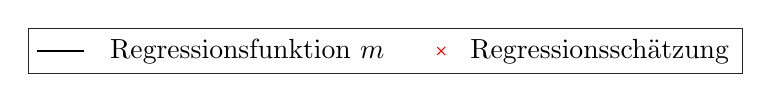
\begin{tikzpicture} 
    \begin{axis}[%
    legend columns=2,
    hide axis,
    xmin=10,
    xmax=50,
    ymin=0,
    ymax=0.4,
    legend style={draw=white!15!black,legend cell align=left,column sep=0.25cm}
    ]
    \addlegendimage{no markers,black}
    \addlegendentry{Regressionsfunktion $m \quad$};
     \addlegendimage{only marks,red,mark=x}
    \addlegendentry{Regressionsschätzung};
    \end{axis}
\end{tikzpicture}}
    \end{subfigure}
     \caption{Approximation der Regressionsfunktion $m(x) = \sin\big(\frac{\pi}{2} \cdot x^2\big)$ durch unseren Neuronale-Netze-Regressionsschätzer mit Parametern $d = 1$, $q = 2$, $R = 10^6$, $a = 3$, $M \in \{2,4,9,16\}$ und $N \in \{2,4,9,16\}$, wobei wir immer Kombinationen von $M$ und $N$ betrachten, sodass $(M + 1)\cdot(N + 1) \approx 51$ gilt.}
    \label{fig:subfig.a.5}
\end{figure}

\clearpage
\section{Vergleich des empirischen $L_2$-Fehlers}

In diesem Abschnitt führen wir nun einen Vergleich des empirischen $L_2$-Fehlers zwischen dem in Abschnitt~\ref{Studie} eingeführten Regressionsschätzer und zwei Standardschätzern durch, die im Verlauf dieses Abschnitts vorgestellt werden.
Die simulierten Daten, welche wir verwenden werden, sehen wie folgt aus:
Wir wählen $X$ gleichverteilt auf $[-2, 2]^d$, wobei $d \in \{1,2\}$ die Dimension des Inputs ist. Mit Gleichung~\eqref{eq:Y} können wir $Y$ darstellen, wobei $m = m_d \colon [-2, 2]^d \to \R$ den Regressionsfunktionen
$$ m_1(x) =  \sin\big(0.2 \cdot x^2\big) + \exp(0.5 \cdot x) + x^3$$
und
$$ m_2(x_0, x_1) = \sin\big(\sqrt[2]{x_0^2 + x_1^2}\big)$$
entspricht. 
Den Skalierungsfaktor $\lambda = \lambda_d > 0$ wählen wir als Interquartilsabstand einer Stichprobe von $m_d(X)$. Für den Rauschfaktor $\sigma$ gilt $\sigma \in \{0.05, 0.1\}.$

Als Nächstes kommen wir zu den Schätzern, die wir in diesem Abschnitt vergleichen möchten. Für die Wahl der Parameter der jeweiligen Schätzer haben wir uns an \cite{kohler19} orientiert.
Der Schätzer \textit{fc\_neural\_1\_estimate} ($m_{n,2}$) ist ein neuronales Netz mit Architektur~$(1,\bk)$, wobei die Anzahl an Neuronen $\bk$ aus der Menge $\mathcal{A} = \{5, 10, 25, 50, 75\}$ stammt. Die Implementation dieses Schätzers erfolgte mithilfe der $Keras$ Bibliothek~\cite{chollet2015keras}. Keras ist eine \emph{High-Level} Anwendungs-Programmierschnittstelle für neuronale Netze in Python. Wir haben uns für Keras entschieden, da diese Bibliothek einfaches und schnelles Erstellen von neuronalen Netzen durch Benutzerfreundlichkeit, Modularität und Erweiterbarkeit ermöglicht. Für das neuronale Netz haben wir die \emph{ReLU} Aktivierungsfunktion $f(x) = \max\{0,x\}$ verwendet. Die Anzahl der Neuronen aus der Menge $\mathcal{A}$ in der verborgenen Schicht ist so gewählt, dass diese zu einem minimalen empirischen $L_2$-Fehler des Schätzers führt.

Unser nächster Schätzer \textit{nearest\_neighbor\_estimate} ($m_{n,3}$) ist ein Nächste-Nachbar-Schät"=zer \cite[Kapitel~7.1]{fahrmeir2009regression}, bei dem die Anzahl an nächsten Nachbarn so aus der Menge~$\{ 2,3,\dots,9\}$ ausgewählt wird, dass dieser zu einem minimalen empirischen $L_2$-Fehler führt. Diesen Schätzer haben wir mithilfe der \emph{Scikit-learn} Bibliothek implementiert \cite{scikit-learn}. Scikit-learn ist eine Bibliothek für maschinelles Lernen in Python, die viele effiziente Werkzeuge für maschinelles Lernen, statistische Modellierung einschließlich Klassifikation und Regression enthält.

Um die Qualität der Schätzung mittels Kennzahlen zu quantifizieren und um diese mit anderen Schätzern zu vergleichen, betrachten wir in Tabelle~\ref{tab:truthTablesm1} und Tabelle~\ref{tab:truthTablesm2} den Interquartilsabstand und den Median des skalierten empirischen $L_2$-Fehlers $\epsilon_{L_2}(m_{n,i})$ der einzelnen Schätzer $m_{n,i}$ von einer Stichprobe von Schätzungen. 

Für die Schätzung von $m_1$ setzen wir: $d = 1$, $N = 3$, $q = 2$, $R = 10^6$, $a = 2$, $M = 2$, da diese Wahl der Parameter bereits sehr gute und schnelle Schätzungen liefert. Für die Schätzung von $m_2$ erhalten wir bereits mit: $d = 2$, $N = 2$, $q = 2$, $R = 10^6$, $a = 2$, $M = 2$ sehr gute Schätzungen.

Wir betrachten ein skaliertes Fehlermaß, da wir die zu schätzenden Regressionsfunktionen~$m_d$ kennen und der Fehler stark von der Komplexität der zu schätzenden Funktion abhängt. Dieses skalierte Fehlermaß ist so zu verstehen, dass wir den empirischen $L_2$-Fehler in Verhältnis zum Median des empirischen $L_2$-Fehlers $\bar{\epsilon}_{L_2}$ des \textit{konstanten Schätzers} setzen. Dieser konstante Schätzer approximiert die Regressionsfunktion mit dem arithmetischen Mittel der Funktionswerte auf dem Trainingsdatensatz. Die Skalierung führt dazu, dass ein großer Fehler eines Regressionsschätzers im Falle, dass der Fehler des konstanten Schätzers klein ist, auf eine noch schlechtere Leistung hindeutet.

Unser Vorgehen zum Vergleich der drei hier betrachteten Regressionsschätzer gestaltet sich wie folgt:
Da die resultierenden skalierten Fehler noch von der Stichprobe von $(X, Y)$ abhängen und um diese Werte besser vergleichen zu können, führen wir die Fehlerberechnung jeweils $50$-mal durch und geben dann den Median und den Interquartilsabstand für die Schätzung der betrachteten Regressionsschätzer aus.
Um diesen skalierten empirischen $L_2$-Fehler in jeder der 50 Iterationen zu bestimmen, gehen wir folgt vor:
Wir erzeugen ein Training-Sample $X_{\text{train}}$ aus Realisierungen von $X$ der Größe $800$ und ein Testing-Sample~$X_{\text{test}}$ der Größe $n = 200$.
Auf dem Training-Sample werden nun auch die Werte $Y_{\text{train}}$ als Realisierung der Zufallsvariable $Y$ über Gleichung~\eqref{eq:Y} bestimmt. Jedem einzelnen dieser Schätzer werden nun die Training-Samples $X_{\text{train}}$ und $Y_{\text{train}}$ zum Lernen bzw.\@ Festlegen der Parameter gegeben. Wir bestimmen als Erstes den $L_2$-Fehler der einzelnen Schätzer $m_{n,i}$ mit $i = 1,2,3$ approximativ durch den empirischen $L_2$-Fehler~$\epsilon_{L_2}(m_{n,i})$ auf der unabhängigen Stichprobe $X_{\text{test}}.$ Mit dem konstanten Schätzer bestimmen wir nun 25-mal den empirischen $L_2$-Fehler auf einer unabhängigen Stichprobe von Realisierungen von $X$ der Größe 200.
Von dieser Stichprobe von Fehlern nehmen wir nun den Median und erhalten so das skalierte Fehlermaß $\epsilon_{L_2}(m_{n,i}) / \bar{\epsilon}_{L_2}.$

%\begin{figure}
%\centering
%%\input{tikzfigure1.tikz}
%\begin{tikzpicture}
%\begin{axis}[x dir=reverse]
%\addplot3 [scatter, only marks]
%  table[x=x, y=y, z=f, col sep=comma] {plotpostpro_sort.csv};
%\end{axis}
%\end{tikzpicture}
%\end{figure}

Wie wir in Tabelle~\ref{tab:truthTablesm1} und Tabelle~\ref{tab:truthTablesm2} anhand des Medians und des Interquartilsabstands des skalierten $L_2$-Fehlers sehen können, übertrifft unserer Neuronale-Netze-Regressions"=schätzer in allen Fällen die Leistung der anderen Schätzer. Diese Schlussfolgerung steht im Einklang mit den Resultaten für den zweidimensionalen Fall aus \cite[Tabel 1]{kohler19} .
\begin{table}
\centering
\begin{tabular}{ |p{5cm}||p{1.7cm} p{2cm}|p{1.7cm} p{2cm}|}
 \hline
 & \multicolumn{4}{|c|}{$m_1$}\\
 \hline
 $\sigma$& $5\%$& & $10\%$ &\\
 \hline
 $\bar{\epsilon}_{L_2,N}$& $13.4482362$ & & $13.3925910$ & \\
 \hline
 \textit{Lageparam.\@ (Streuungsmaß) }&  Median &(IQA) &  Median &(IQA)   \\
 \hline
new\_neural\_network\_estimate & $\mathbf{2.482\textbf{e-}05}$& $\mathbf{(1.612\textbf{e-}05)}$   & $\mathbf{6.908\textbf{e-}05}$&$\mathbf{ (3.936\textbf{e-}05)}$  \\
 fc\_neural\_1\_estimate & $4.384\text{e-}04$&$(2.14\text{e-}03)$ &   $7.261\text{e-}04$&$(4.57\text{e-}03)$ \\
 nearest\_neighbor\_estimate & $2.9527\text{e-}04$&$(9.312\text{e-}05)$ & $9.0864\text{e-}04$&$(2.895\text{e-}04)$\\
 \hline
\end{tabular}
    \caption{Median und IQA von $50$ skalierten empirischen $L_2$-Fehlern für Schätzungen von $m_1$.}
     \label{tab:truthTablesm1}   
\end{table}

    \begin{table}
\centering
\begin{tabular}{ |p{5cm}||p{1.7cm} p{2cm}|p{1.7cm} p{2cm}|}
 \hline
 & \multicolumn{4}{|c|}{$m_2$}\\
 \hline
 $\sigma$& $5\%$ & & $10\%$ &  \\
 \hline
 $\bar{\epsilon}_{L_2,N}$& $0.0324$ & & $0.0311$ & \\
 \hline
 \textit{Lageparam.\@ (Streuungsmaß)}&  Median &(IQA) &  Median &(IQA)   \\
 \hline
 new\_neural\_network\_estimate & $\mathbf{0.003961}$ & $\mathbf{(0.000932)}$   & $\mathbf{0.00431}$ & $\mathbf{(0.000973)}$  \\
 fc\_neural\_1\_estimate & $0.0257$ & $(0.3803)$ &   $0.0559$ &  $(0.52033)$ \\
 nearest\_neighbor\_estimate & $0.01616$ & $(0.005906)$ &$0.01763$ & $(0.007081)$\\
 \hline
\end{tabular}
    \caption{Median und IQA von $50$ skalierten empirischen $L_2$-Fehlern für Schätzungen von $m_2$.}
    \label{tab:truthTablesm2}   
\end{table}
